\documentclass[10pt,aspectratio=169]{beamer}
\usetheme[
%%% options passed to the outer theme
%    hidetitle,           % hide the (short) title in the sidebar
    hideauthor,          % hide the (short) author in the sidebar
%    hideinstitute,       % hide the (short) institute in the bottom of the sidebar
%    shownavsym,          % show the navigation symbols
%    width=2cm,           % width of the sidebar (default is 2 cm)
    hideothersubsections,% hide all subsections but the subsections in the current section
%    hideallsubsections,  % hide all subsections
    right               % right of left position of sidebar (default is right)
%%% options passed to the color theme
%    lightheaderbg,       % use a light header background
  ]{AAUsidebar}

% If you want to change the colors of the various elements in the theme, edit and uncomment the following lines
% Change the bar and sidebar colors:
%\setbeamercolor{AAUsidebar}{fg=red!20,bg=red}
%\setbeamercolor{sidebar}{bg=red!20}
% Change the color of the structural elements:
%\setbeamercolor{structure}{fg=red}
% Change the frame title text color:
%\setbeamercolor{frametitle}{fg=blue}
% Change the normal text color background:
%\setbeamercolor{normal text}{bg=gray!10}
% ... and you can of course change a lot more - see the beamer user manual.


\usepackage[utf8]{inputenc}
\usepackage[english]{babel}
\usepackage[T1]{fontenc}
\usepackage{booktabs}
\usepackage{multimedia}
\usepackage{multicol}
\usepackage{color}
\usepackage{listings}
\usepackage{listings-golang}
\usepackage{yaml}
\usepackage{tikz,pgfplots}
\usepackage{xcolor}
\definecolor{listinggray}{gray}{0.9}
\definecolor{lbcolor}{rgb}{0.9,0.9,0.9}
\lstset{
	backgroundcolor=\color{listbackground},
	tabsize=4,
	rulecolor=,
    frame=single,
	language=matlab,
        basicstyle=\scriptsize,
        upquote=true,
        aboveskip={1.5\baselineskip},
        columns=fixed,
        showstringspaces=false,
        extendedchars=true,
        breaklines=true,
        prebreak = \raisebox{0ex}[0ex][0ex]{\ensuremath{\hookleftarrow}},
        % frame=single,
        showtabs=false,
        showspaces=false,
        showstringspaces=false,
        identifierstyle=\ttfamily,
        keywordstyle=\color[rgb]{0,0,1},
        commentstyle=\color[rgb]{0.133,0.545,0.133},
        stringstyle=\color[rgb]{0.627,0.126,0.941},
}
\definecolor{feupblue}{RGB}{140,45,25}
\definecolor{listbackground}{HTML}{D8F0FB}
\definecolor{color6}{RGB}{242,130,65}
\definecolor{color1}{RGB}{146,212,245}
\definecolor{color2}{RGB}{78,184,237}
\definecolor{color3}{RGB}{2,154,229}
\definecolor{color4}{RGB}{1,108,160}
\definecolor{color5}{RGB}{0,54,92}
% Or whatever. Note that the encoding and the font should match. If T1
% does not look nice, try deleting the line with the fontenc.
\usepackage{helvet}

% colored hyperlinks
\newcommand{\chref}[2]{%
  \href{#1}{{\usebeamercolor[bg]{AAUsidebar}#2}}%
}

\title[Identificação de Tonalidade]% optional, use only with long paper titles
{Identificação de Tonalidade em ficheiros MIDI}
\subtitle{Trabalho de Grupo 3}  % could also be a conference name


\date{Maio 2021}

\author[Authors in sidebar] % optional, use only with lots of authors
{
  Diogo Remião 201706373 \\
  José Miguel Pinheiro 201705172
}
% - Give the names in the same order as they appear in the paper.
% - Use the \inst{?} command only if the authors have different
%   affiliation. See the beamer manual for an example

\institute[
%  {\includegraphics[scale=0.2]{aau_segl}}\\ %insert a company, department or university logo
  Sistemas Multimédia \\
  FEUP
] % optional - is placed in the bottom of the sidebar on every slide
{% is placed on the title page
  Sistemas Multimédia \\
  FEUP

  %there must be an empty line above this line - otherwise some unwanted space is added between the university and the country (I do not know why;( )
}


% specify a logo on the titlepage (you can specify additional logos an include them in
% institute command below
\pgfdeclareimage[height=1.5cm]{titlepagelogo}{AAUgraphics/feup_logo} % placed on the title page
%\pgfdeclareimage[height=1.5cm]{titlepagelogo2}{graphics/aau_logo_new} % placed on the title page
\titlegraphic{% is placed on the bottom of the title page
  \pgfuseimage{titlepagelogo}
%  \hspace{1cm}\pgfuseimage{titlepagelogo2}
}


\begin{document}
% the titlepage
{\aauwavesbg%
\begin{frame}[plain,noframenumbering] % the plain option removes the sidebar and header from the title page
  \titlepage
\end{frame}}
%%%%%%%%%%%%%%%%

% TOC
\begin{frame}{Agenda}{}
    \begin{multicols}{2}
        \setcounter{tocdepth}{2}
        \tableofcontents
    \end{multicols}
\end{frame}
%%%%%%%%%%%%%%%%
\section*{Caracterização geral da simulação}

%sistemas
\noindent
Este \textit{Call center} tem dois sistemas separados:
\begin{itemize}
    \item Sistema GP, que atende todas as chamadas e reencaminhada chamadas para o sistema AS se necessário
    \item Sistema AS, que atende as chamadas de carácter específico reencaminhadas pelo sistema GP
\end{itemize}

%parametros
\noindent
Definimos os seguintes parâmetros de funcionamento do \textit{Call center}:
\begin{itemize}
    \item Nº de servidores no sistema GP
    \item Nº de servidores no sistema AS
    \item Tamanho da fila de espera no sistema GP (infinita no sistema AS)
\end{itemize}


%chamadas
\noindent
Sendo esta uma simulação de um \textit{Call center}, duas situações podem acontecer:
\begin{itemize}
    \item 30\% de probabilidade de uma chamada apenas precisar de ser atendida no sistema GP.
    \item 70\% de probabilidade de uma chamada precisar de ser no sistema GP e depois no sistema AS.
\end{itemize}


%eventos
\noindent
Distinguem-se 3 tipos de eventos no sistema:
\begin{itemize}
    \item CHEGADA: Uma chamada que chega a um sistema, sem discriminação do seu tipo.
    \item PARTIDA\_GP: Uma chamada que é atendida no sistema GP e depois sai do sistema.
    \item PARTIDA\_AS: Uma chamada que é atendida no sistema GP e entra no sistema AS / Chamada que é atendida no AS
\end{itemize}

As distinção entre PARTIDA\_GP e PARTIDA\_AS é apenas relevante no sistema GP. No sistema AS, faz-se uma abstração para apenas PARTIDA.

Cada evento tempo um \textit{timestamp} associado.
No evento de \textbf{CHEGADA}, define o momento em que chegou.
Nos de \textbf{PARTIDA}, o momento em que partiu.
Este valores são gerados conforme indicado no guião.
\newline

%listas
\noindent
A \textbf{lista\_eventos\_gp} é uma fila onde serão guardados todos os eventos que chegam ao sistema GP.
A \textbf{lista\_espera\_gp} é uma fila onde serão guardados todos os eventos que estão num determinando momento na fila de espera para serem processados pelo sistema GP.
Um evento é colocado na fila de espera quando todos servidores estão ocupados.
Se a fila estiver cheia, a chamada é considerada como perdida e removida.

A \textbf{lista\_eventos\_as} e a \textbf{lista\_espera\_as} têm a mesma funcionalidade mas para o sistema AS.
Um evento é colocado na fila de espera quando o os servidores estão ocupados.
A fila de espera é infinita, pelo que não haverá chamadas perdidas.

\section*{Descrição do funcionamento do algoritmo}

\begin{figure}[H]
    \centering
    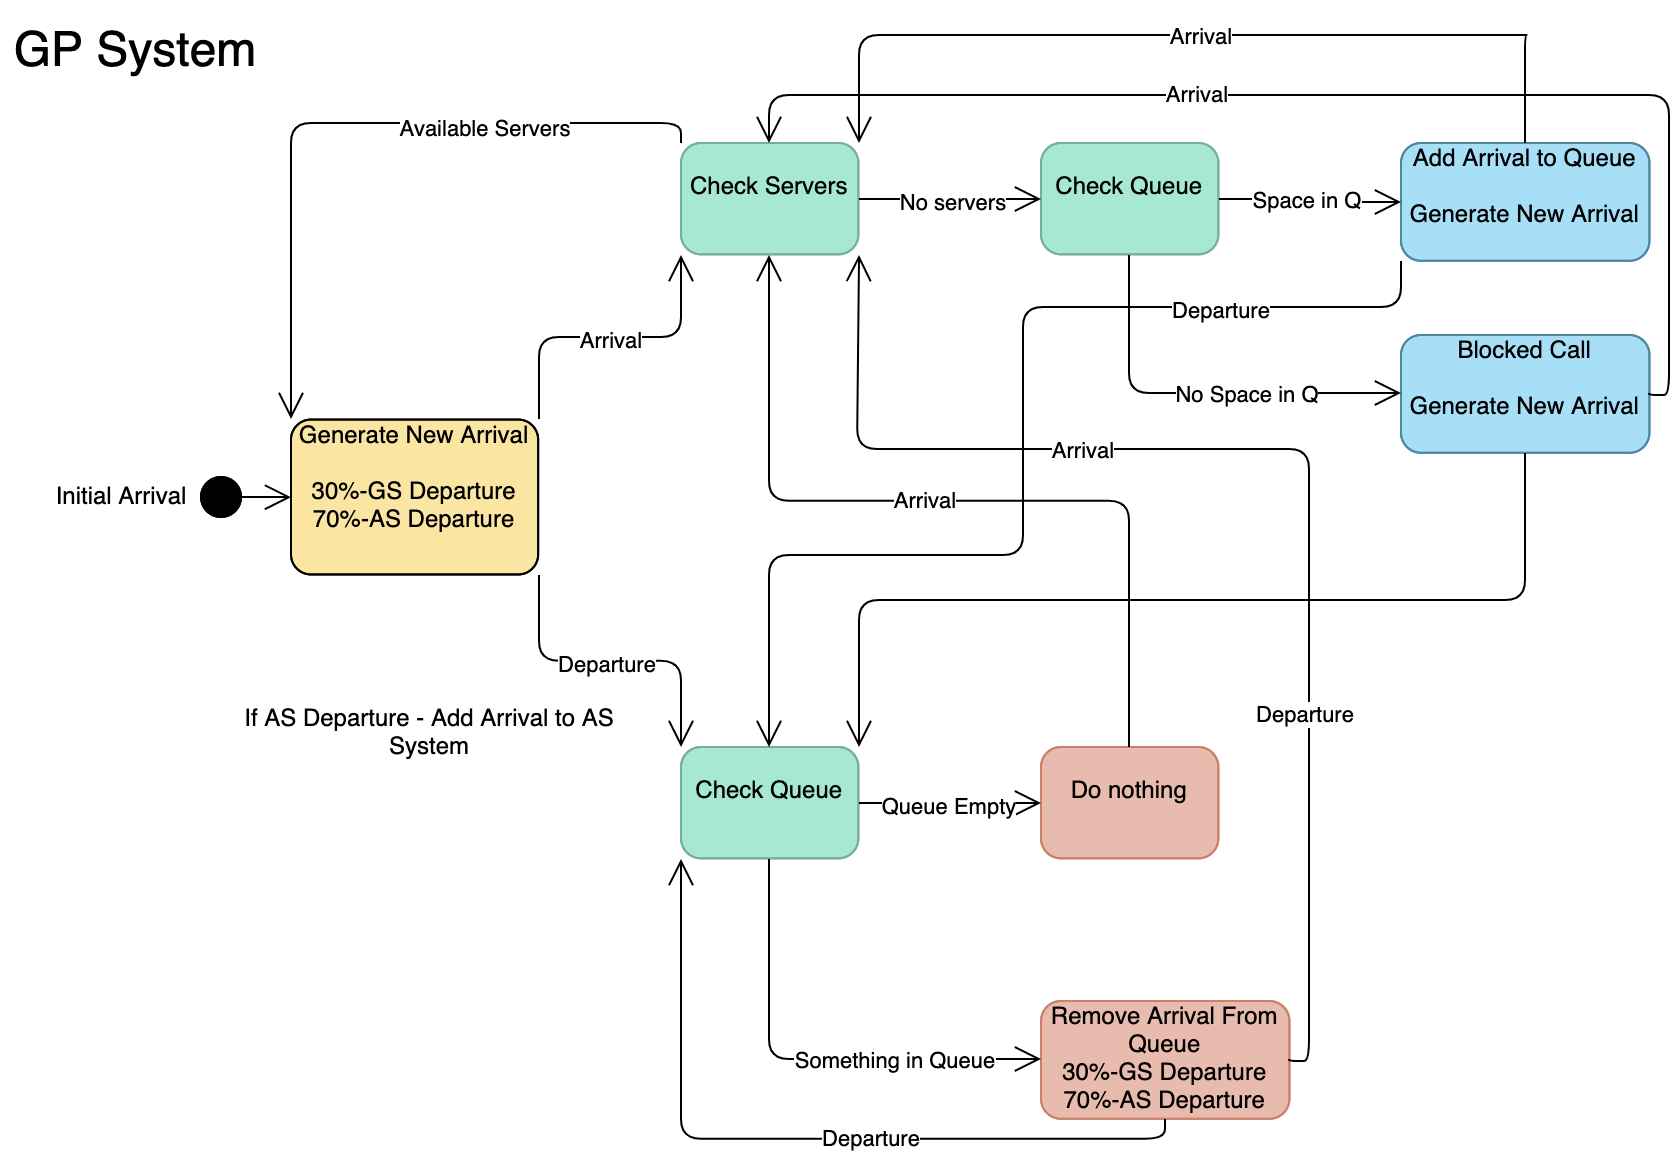
\includegraphics[width=.9\linewidth]{figs/intro/sm_gp.png}
    \caption{Máquina de estados do Sistema General Purpose}
    \label{fig:sm_gp}
\end{figure}

A figura \ref{fig:sm_gp} é uma máquina de estados que representa o algoritmo do \textbf{sistema GP}.
Primeiro verifica-se o tipo de evento que está na \textbf{lista\_eventos\_gp}.

Se o evento for de \textbf{CHEGADA}, verifica-se o estado do sistema.
Se os servidores estivem ocupados, verifica-se a fila de espera.
Se esta estiver livre, esse evento é colocado na \textbf{lista\_espera\_gp}.
Caso contrário é bloqueado.
Novas \textbf{CHEGADAS} são sempre geradas quando se processa uma \textbf{CHEGADA}.

Se o evento for de \textbf{PARTIDA}, verifica-se se há algum evento na \textbf{lista\_espera\_gp}.
Se houver, começa-se imediatamente a processar esse evento, gerando uma nova \textbf{PARTIDA}.
Caso contrário, passa-se para o próximo evento na \textbf{lista\_eventos\_gp}.

Por fim, considera-se que uma \textbf{CHEGADA} é gerada no \textbf{sistema AS} quando é processada uma \textbf{PARTIDA\_AS}.


\noindent
\newline
O princípio de funcionamento do sistema AS é semelhante, ilustrado na figura \ref{fig:sm_as}. Destaca-se alguma diferenças.


As \textbf{CHEGADAS} não são geradas no \textbf{sistema AS}, mas sim no \textbf{sistema GP}, pelo que o sistema pode ficar inativo, algo que não acontece com o \textbf{sistema GP}.
Além disso, não existe a risco de uma chamada ser bloqueada pois a fila é infinita.
A \textbf{lista\_eventos\_as} é constantemente verificada para detetar se alguma chamada foi reencaminhada para ser atendida pela sistema. Quando o sistema fica \textit{idle}, volta a este estado.

As \textbf{PARTIDAS} são geradas também quando uma CHEGADA é processada, no entanto a distribuição temporal é diferente das duas partidas do sistema GP.

\begin{figure}[H]
    \centering
    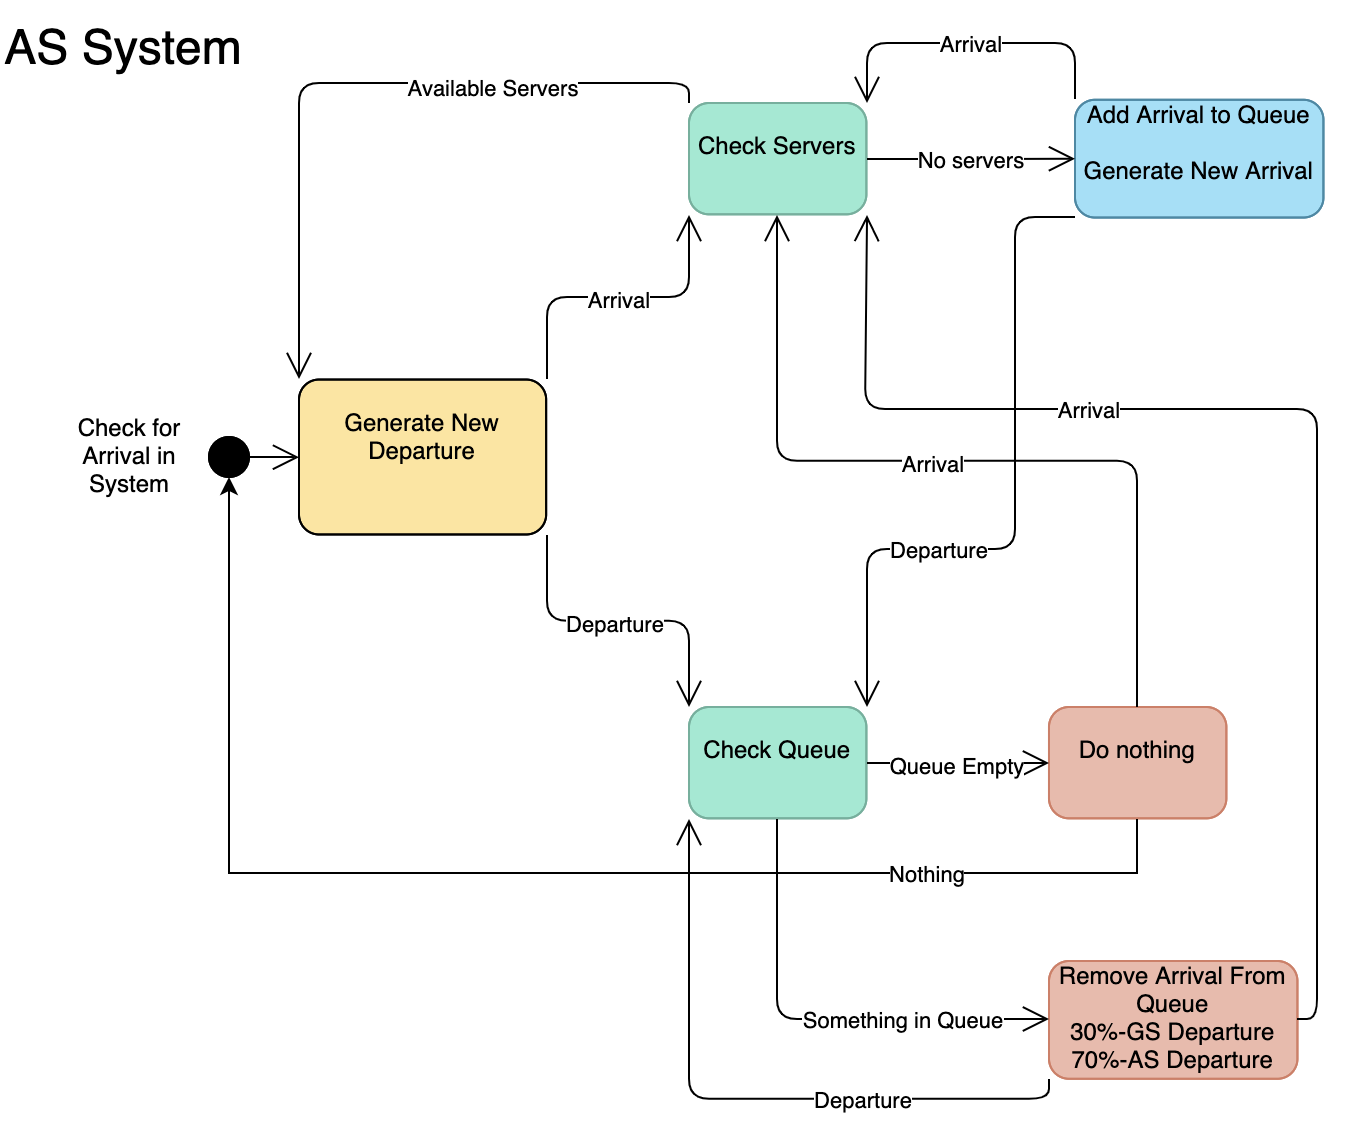
\includegraphics[width=.7\linewidth]{figs/intro/sm_as.png}
    \caption{Máquina de estados do Sistema Area Specific}
    \label{fig:sm_as}
\end{figure}

\section*{Estimativa do tempo de espera}

De forma a puder fornecer uma previsão do tempo de espera a cada chamada que chega, é necessário adotar um algoritmo de \textit{running average}.
Este algoritmo permite o calculo dinâmico da média do tempo de espera a cada chamada que chega, atualizando a cada iteração.

A estimativa do tempo de espera começa a 1. Quando uma chamada chega, duas situações podem acontecer:
\begin{itemize}
    \item Chamada é imediatamente atendida, pelo que o delay é 0 segundos.
    \item Chamada é colocada na fila de espera. O delay é calculado no momento em que a chamada sai da fila de espera.
\end{itemize}

Quando um novo valor de delay é obtido, uma nova média é calculada.
Por exemplo, com um delay de 60 segundos, a nova média será $\frac{0+60}{2}=30s$.
Quando uma nova chamada chegar, a estimativa de tempo de espera apresentada será de 30 segundos.
A cada iteração, este valor é atualizado.
Como este sistema tende para a estabilidade, este valor aproxima-se para um valor constante, que vai fornecer uma previsão mais sólida quantas mais chamadas forem atendidas.


\section*{Resultados da simulação}

De modo a garantir os objetivos de performance mínimos, necessitamos de pelo menos \textbf{4 Servidores GP}, \textbf{2 Servidores AS} e \textbf{Fila de Espera GP de tamanho 2}.
Os seguintes parâmetros foram obtidos:
\begin{center}
    \begin{tabular}{||c|c c||} 
    \hline
    Parâmetro & Mínimo & \textbf{Obtido} \\
    \hline\hline
    Delay Prob & 30\% & \textbf{12.83\%}\\ 
    \hline
    Blocked Prob & 2\% & \textbf{1.35\%}\\
    \hline
    Avrg Delay GS& 30s & \textbf{23.4s}\\
    \hline
    Avrg Delay Total & 60s & \textbf{24s} \\
    \hline
   \end{tabular}
\end{center}

O \textit{Bottleneck} deste sistema é o \textbf{Avrg Delay GS}, que está muito mais próximo do limite do que os restantes parâmetros.
Um relaxamento deste parâmetro para 40 segundo permitia que fosse utilizado apenas 3 servidores GP.

Com estes parâmetros, foram gerados histogramas que representam a distribuição dos atrasos e dos erros de previsão.

\begin{figure}[H]
    \centering
    \begin{subfigure}[b]{0.49\textwidth}
        \centering
    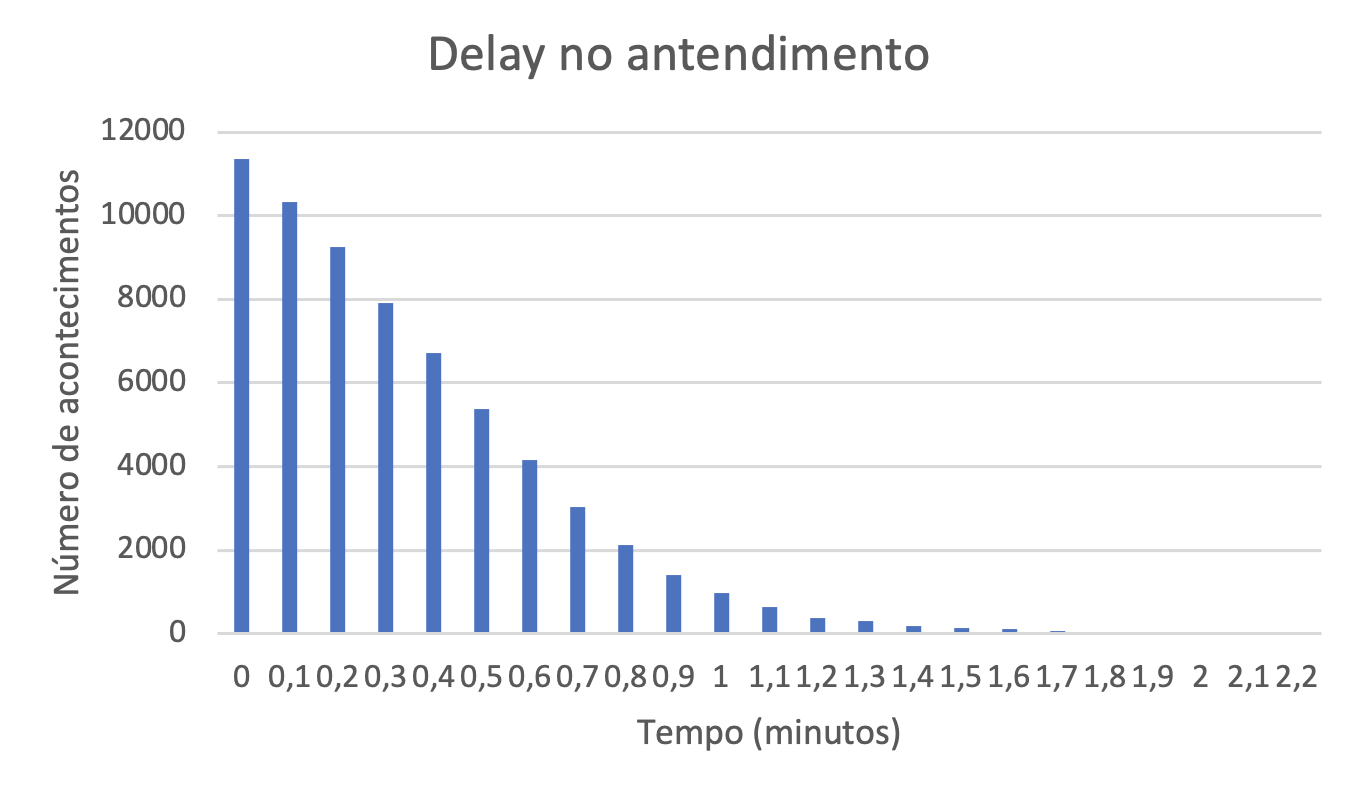
\includegraphics[width=\linewidth]{figs/intro/histo_delay.png}
    \caption{Distribuição dos delays no sistema}
    \label{fig:histo_delay}
    \end{subfigure}
    \hfill
    \begin{subfigure}[b]{0.5\textwidth}
        \centering
    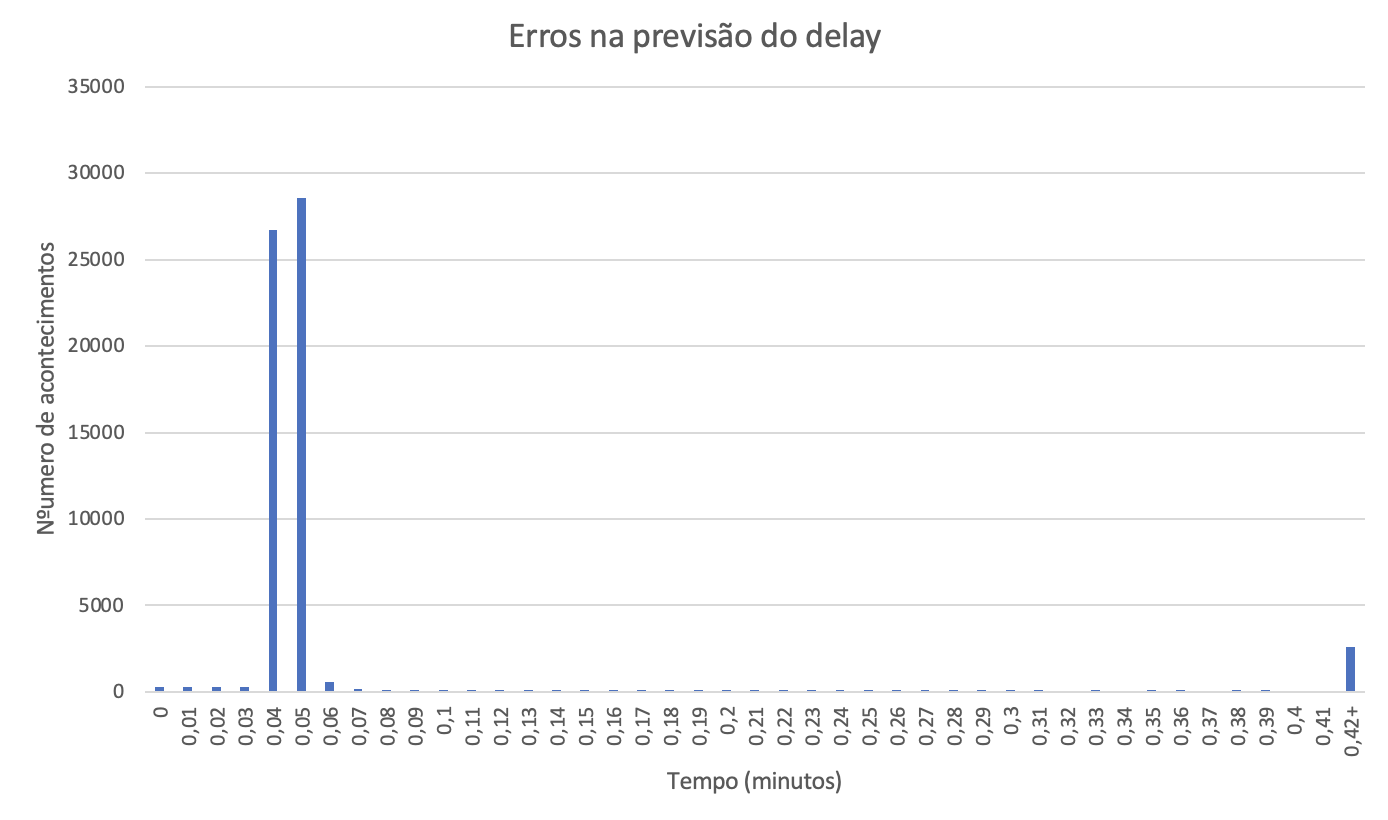
\includegraphics[width=\linewidth]{figs/intro/histo_erro.png}
    \caption{Distribuição do erro de previsão no sistema}
    \label{fig:histo_erro}
    \end{subfigure}
       \label{fig:histogramas}
\end{figure}

A distribuição dos dos \textit{Delays} aproxima-se de uma distribuição exponencial, pois este sistema é estável, ou seja, $\rho<1$.
Se $\rho>1$, esta distribuição seria crescente pois o tempo de espera iria aumentar com o tempo. Os delays 0 não estão representados.

Uma analíse do histograma dos erros indica que grande parte dos erros foi na ordem dos 0.04-0.06 segundos, que é sensivelmente o valor médio de atraso.
Mais uma vez, o facto do sistema ser estável fez com que os erros obtidos fossem da ordem da média.

\section*{Análise de Sensibilidade e Estimador}

\begin{figure}[H]
    \begin{floatrow}
    \ffigbox{%
    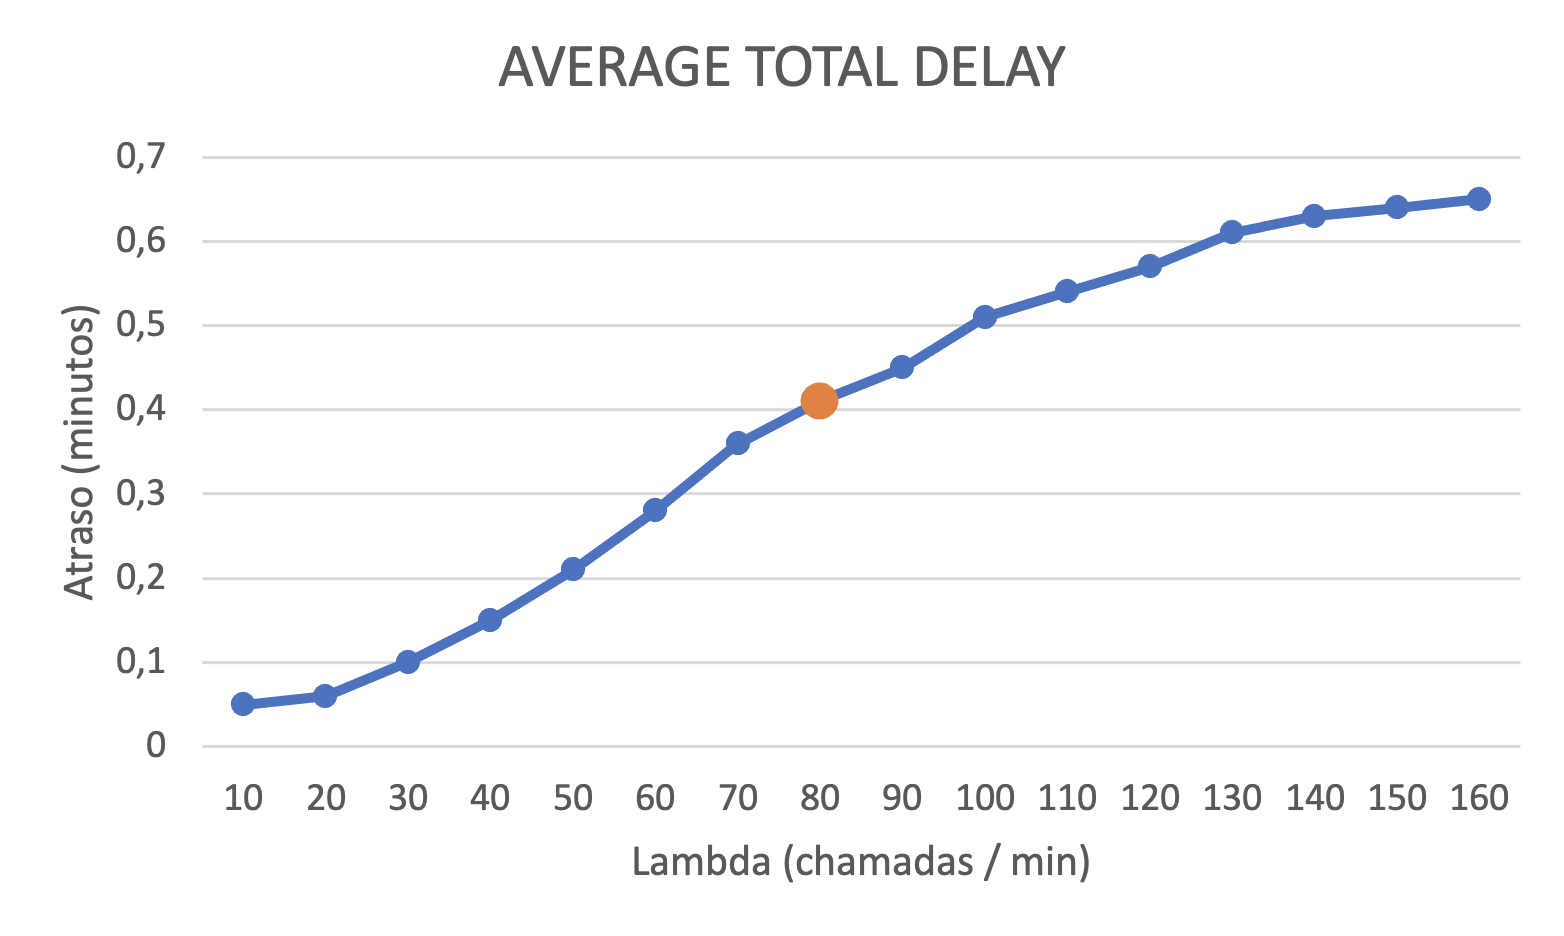
\includegraphics[width=.9\linewidth]{figs/intro/total_delay.png}
    }{%
    \caption{Total Delay time com variação da frequência de chegadas}
    }
    \capbtabbox{%
    \begin{tabular}{||c|c||} 
        \hline
        Intervalo de Confiança & 90\% \\
        \hline
        Número de Amostras & 30 \\
        \hline
        Graus de Liberdade & 29 \\
        \hline
        t (Student) & 1.6973 \\
        \hline
        Média & 0.410105 \\
        \hline
        Desvio Padrão & 0.005534535\\
        \hline
        Limite Inferior & 0.408389941 \\
        \hline
        Limite Superior & 0.411820059 \\
        \hline
       \end{tabular}
    }{%
    \caption{Estimador do Average Total Wait Time com intervalo de confiança de 90\% - 2 Tail}
    }
    \end{floatrow}
\end{figure}


A figura 4 mostra a relação entre a \textit{Arrival Rate} e o Atraso do sistema.
Observamos, como esperado, que o atraso tende para 0 à medida que se diminúi a \textit{Arrival Rate}.

À medida que o valor aumenta, o atraso tendo para um valor próximo de 0.65 minutos.
Isto deve-se ao facto da fila de espera ter tamanho limite.
O tempo que uma chamada tem que esperar se estiver no fim da fila não aumenta pois tem sempre o mesmo número de chamadas à sua frente.
O que aumenta é a probabilidade de perder a chamada. É deste modo de esperar este comportamento.

Também foi calculado um estimar para o Average Total Wait Time com base em 30 amostras do parâmetro.


\section{Fundamentos Teóricos}
\begin{frame}{Fundamentos Teóricos}{}
\begin{itemize}
    \item Tonalidade
    \begin{itemize}
        \item Cifra
        \item Escalas / Acordes / Cadências
    \end{itemize}
    \item Tonalidades Próximas
    \begin{itemize}
        \item Relativa / Dominante / Sub-Dominante / Paralela
    \end{itemize}
    \item Técnicas de Identificação
\end{itemize}
\end{frame}

\subsection{Tonalidade}
\begin{frame}{Fundamentos Teóricos}{Tonalidade}
    \begin{columns}[]
        \begin{column}{.4\textwidth}
            \begin{itemize}
            \item O que é a tonalidade
            \item Cifra
            \item Derivações
            \begin{itemize}
                \item Escala
                \item Acordes
                \item Cadências
            \end{itemize}
            \end{itemize}
        \end{column}
        \begin{column}{.6\textwidth}
            \begin{figure}
                
\includegraphics[width=.9\textwidth]{figs/escala.png}
            \end{figure}
            \vspace{-1cm}
            \begin{figure}
                
\includegraphics[width=.9\textwidth]{figs/acorde.png}
            \end{figure}
        \end{column}
    \end{columns}
\end{frame}

\subsection{Tonalidades Próximas}
\begin{frame}{Fundamentos Teóricos}{Tonalidades Próximas}
    \begin{columns}[]
        \begin{column}{.5\textwidth}
            \begin{itemize}
            \item Tonalidades Próximas / Afastadas
            \item Tónica
            \item Relativa
            \begin{itemize}
                \item Maior
                \item Menor
            \end{itemize}
            \item Dominante
            \item Sub-Dominante e Relativas
            \end{itemize}
        \end{column}
        \begin{column}{.5\textwidth}
            \begin{figure}
                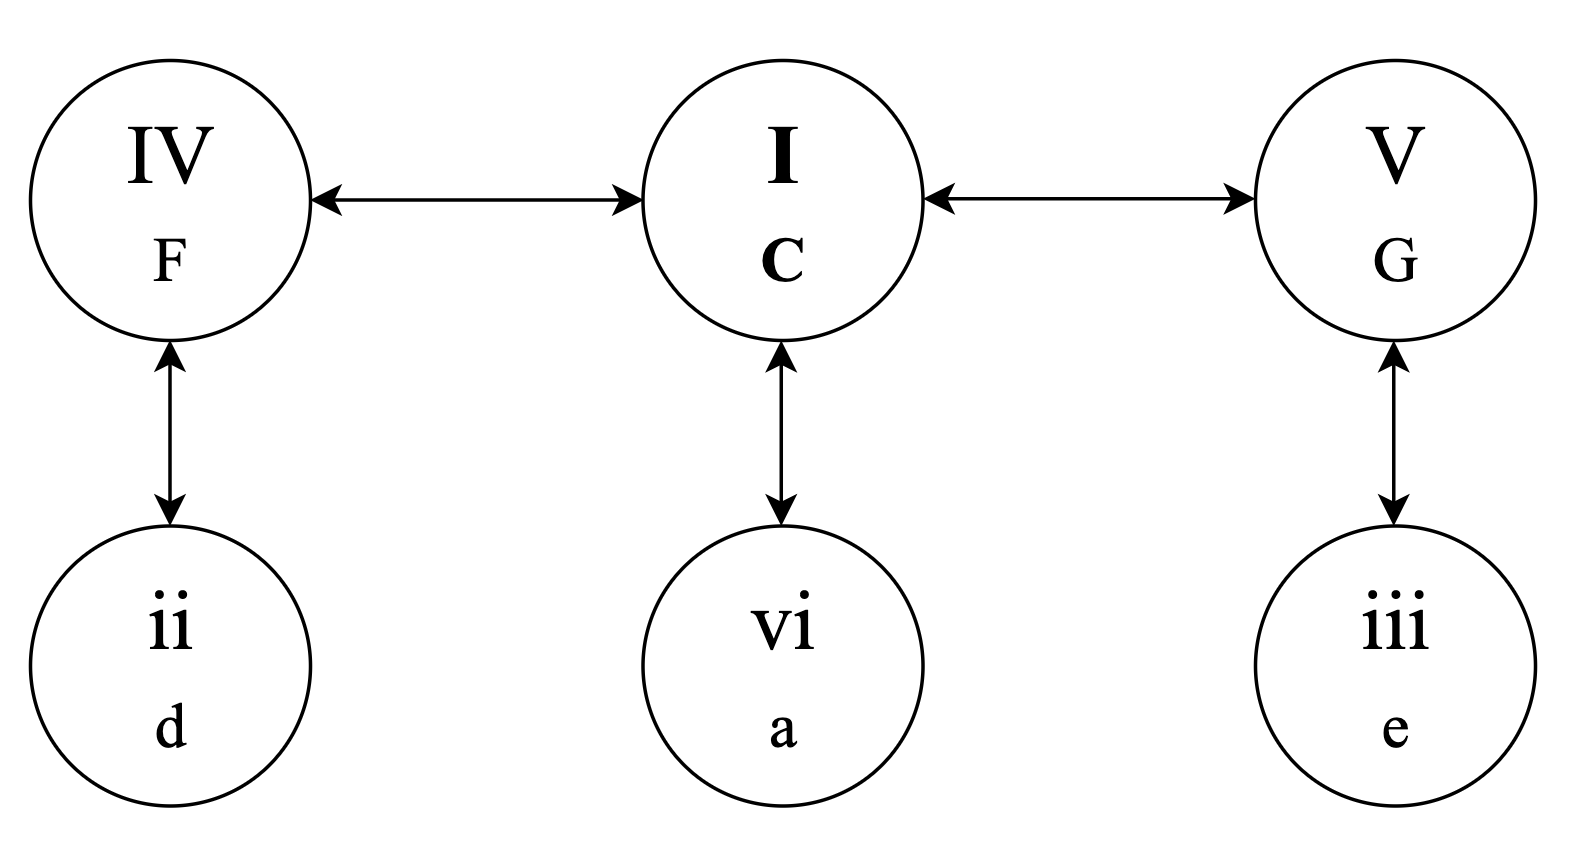
\includegraphics[width=.9\textwidth]{figs/modulacoes.png}
            \end{figure}
        \end{column}
    \end{columns}
\end{frame}

\subsection{Técnicas de Identificação}
\begin{frame}{Fundamentos Teóricos}{Técnicas de Identificação}
    \begin{columns}[]
        \begin{column}{.4\textwidth}
            \begin{itemize}
            \item Cifra
            \item Alterações (Sustenido e bemol)
            \item Progressões Harmónicas - Cadências
            \end{itemize}
        \end{column}
        \begin{column}{.6\textwidth}
            \begin{figure}
                
\includegraphics[width=.95\textwidth]{figs/schubert.png}
            \end{figure}
        \end{column}
    \end{columns}
\end{frame}

\section{Método}
\begin{frame}{Método}{}
    \begin{itemize}
        \item Algoritmo de Krumhansl-Schmukler
        \item Key Profiles
        \begin{itemize}
            \item Krumhansl
            \item Variações: Temperley / Aarden / Bellman / Simple (Craig)
        \end{itemize}
        \item Exemplo
    \end{itemize}
\end{frame}

\subsection{Algoritmo de Krumhansl-Schmukler}
\begin{frame}{Método}{Algoritmo de Krumhansl-Schmukler}
    \begin{columns}[]
        \begin{column}{.5\textwidth}
            \begin{itemize}
                \item Baseado em perfis tonais (\textit{Key Profiles})
                \item Construção de uma distruibuição representativa da presença de cada nota
                \begin{itemize}
                    \item Temporal e variável com a métrica escolhida
                \end{itemize}
                \item Autocorrelação com cada perfil tonal
                \begin{itemize}
                    \item Perfil com maior correlação é o escolhido
                \end{itemize}
            \end{itemize}
        \end{column}
        \begin{column}{.5\textwidth}
            \begin{figure}
                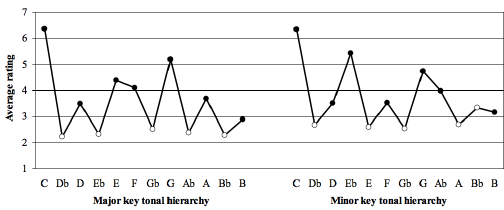
\includegraphics[width=.9\textwidth]{figs/key_profiles_C.png}
            \end{figure}
        \end{column}
    \end{columns}
\end{frame}

\subsection{Key Profiles}
\begin{frame}{Método}{Key Profiles}
    \begin{itemize}
        \item Krumhansl-Schmukler \& Kessler
        \begin{itemize}
            \item Análise subjetiva com voluntários 
            \item Quão bem uma nota soa num elemento musical de uma tonalidade (Escala, Cadência, etc)
            \item Contrução de um perfil tonal para todas as tonalidades maiores e outra para as menores
        \end{itemize}
        \item Temperley
        \item Bellman e Aarden
        \item Simple (Craig)
    \end{itemize}
\end{frame}

\subsection{Exemplo}
\begin{frame}{Método}{Exemplo}
    \begin{columns}[]
        \begin{column}{.5\textwidth}
            \begin{itemize}
                \item Melodia "Yankee Doodle"
                \item Construção da distruibuição
                \item Correlação com os perfis de Krumhansl
                \item Melhor previsão - G Major (0.693)
                \begin{itemize}
                    \item D Major (0.485)
                    \item E Minor (0.398)
                    \item G Minor (0.394)
                \end{itemize}
            \end{itemize}
        \end{column}
        \begin{column}{.5\textwidth}
            \begin{figure}
                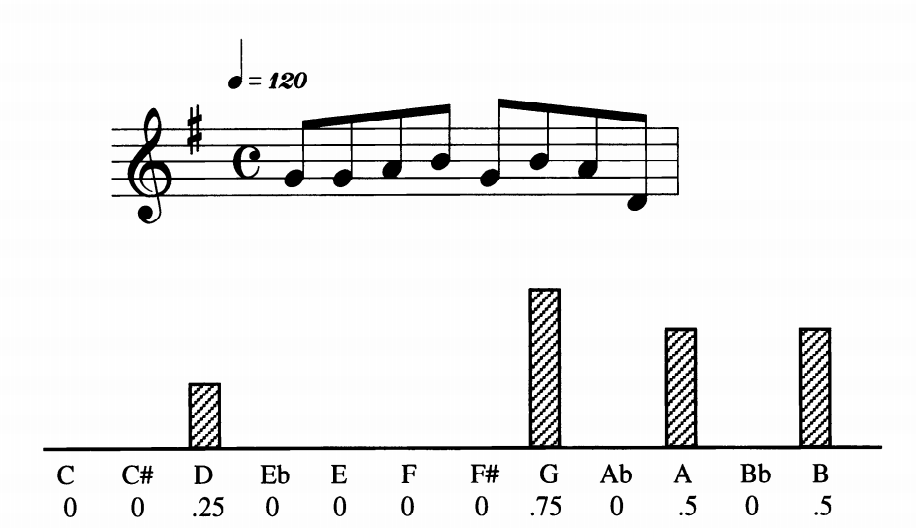
\includegraphics[width=.9\textwidth]{figs/yankee_song.png}
            \end{figure}
        \end{column}
    \end{columns}
\end{frame}
\section{Implementation} \label{sec:implementation}

Having described the algorithm, the next step is to implement it programmatically.
This is because if we want to obtain a significant number of results, doing calculations by hand would be impractical.

The implementation was done in Python, a high level programming language, with lots of libraries and tools for multimedia projects.
We made use of the library \textit{Music21}, a Python-based toolkit for computer-aided musicology \cite{music21}.

This library has a key determination algorithm implemented based on the \textit{Krumhansl-Schmuckler} key determination algorithm.
This is the one we will be making use in this project.

One advantage of this library is that it allows to specify which key-profiles to use when calculation the correlation with the sample.
This will allow us to compare different key profiles and their respective accuracy relatively easily.
For the purpose of the project, we will be explaining in relative detail how to use this library, detailing some classes and functions crucial in this project.

\subsection {music21.stream}

The class \textit{music21.stream} is the fundamental container in \textit{music21}.
It is in this class where objects may be ordered and/or placed in time based on offsets from the start of this container.
This means that it basically encodes music elements on a time-based system, effectively creating a file system that the rest of the library can understand.

Although it is possible to "manually" create a \textit{Stream}, defining which notes are to be played, as well as their time-frame, this is not necessary nor recommended.
What we will be doing in converting a music file into a \textit{Stream} using the function \textit{music21.converter.parse}.

This function accepts a number of symbolic music files, files where the data is structured, and therefore well defined if we know how to read it.
A few examples can be named like MusicXML, MuseData, Humdrum and most importantly, MIDI.

What is consistent amongst all these file types is that, although they store musical data, \textbf{none of them are in fact audio files}.
Although audio files, such as MP3 and WAV, enables us to play music in virtually any device, it does not contain any information regarding what is actually being played, 
i.e, we do not know whether a piano or a flute is playing simply by reading the file. This makes it very difficult to extract information like which notes are being played,
which is the essence of key determination for example.

For this matter, we use file types like MIDI, where all this information is available directly, simplifying significantly the process.
By parsing a MIDI file into a \textit{Stream}, we are know able to make use of the library's analyses function.
It is important to note that some equalization in applied in order to improve the algorithm's efficiency.
However, most excerpts will be unaffected as this equalization is done using a very high tempo subdivision.

\subsection{music21.analysis.discrete.KeyWeightKeyAnalysis} \label{sec:analysis_discrete}

Once we have created a \textbf{Stream} based on a MIDI file, we can now apply analysis tools to obtain different parameters.
One of such tools is the \textit{KeyWeightKeyAnalysis}, the implementation of the key determination algorithm.

To be precise, this class does not exist, i.e, you cannot define an object using this class. It is what is called a base class.
This means that for example classes \textit{...discrete.a} and \textit{...discrete.b}, both subclasses of \textit{...discrete.KeyWeightKeyAnalysis},
inherit the same base functions, although they can have specific functions for them.

The subclasses in this case will different key-profiles alternatives that can be applied in the algorithm:
\begin{itemize}
    \item SimpleWeights - Implementation of simple weights by Craig Sapp \cite{sapp2011computational}
    \item AardenEssen - Implementation of Aarden-Essen weightings \cite{aarden2003dynamic}
    \item BellmanBudge - Implementation of Bellman-Budge weightings \cite{bellmann2005determination}
    \item KrumhanslSchmuckler - Implementation of Krumhansl-Schmuckler/Kessler weightings \cite{krumhansl2001cognitive}
    \item TemperleyKostkaPayne - Implementation of Temperley-Kostka-Payne weightings \cite{Temperley2004Musicp}
\end{itemize}

Like mentioned before, this subclasses output a different correlation value as they make use of different key profiles.

Although not necessary, it is possible to see which profiles are being use for both major and minor keys in each implementation, by making use of the function \textit{KeyWeightKeyAnalysis.getWeights(weightType)}.
For example, this is the output of the Krumhansl-Schmuckler/Kessler weightings, represented in Figure \ref{fig:key_profiles_c}:

\begin{lstlisting}[language=bash]
    Major Key profile [6.35, 2.23, 3.48, 2.33, 4.38, 4.09, 2.52, 5.19, 2.39, 3.66, 2.29, 2.88]
    Minor Key profile [6.33, 2.68, 3.52, 5.38, 2.6, 3.53, 2.54, 4.75, 3.98, 2.69, 3.34, 3.17]
\end{lstlisting}

\subsection{music21.stream.analyze}

Although we can do the analysis by calling \ref{sec:analysis_discrete}, it is easier to simply call \textit{stream.analyze(arg)}.
This function runs a particular analytical method on the contents of the specified stream to find its key in this case, essentially calling \textit{music21.analysis.discrete.KeyWeightKeyAnalysis} functions.
For example, \textit{stream.analyze('key')} would output the prediction based on the implementation of Krumhansl-Schmuckler/Kessler weightings, which is the default one.
Making use of the subclass \textit{music21.analysis.discrete.analyzeStream}, we can specify which implementation we want to use.
This subclass matches the argument string with the implementations available:
\begin{itemize}
    \item analysis.discrete.analyzeStream(s, 'Krumhansl') = stream.analyze('Krumhansl') - Outputs prediction based on Krumhansl profiles
    \item analysis.discrete.analyzeStream(s, 'Temperley') = stream.analyze('Temperley') - Outputs prediction based on Temperley profiles
\end{itemize}

\subsection{music21.key.Key} \label{sec:key}

Independently of the method used to make the prediction the output will be an object of the class \textit{music21.key.Key}.
As described in the documentation, "Note that a key is a sort of hypothetical/conceptual object.
It probably has a scale (or scales) associated with it and a KeySignature, but not necessarily".

The \textbf{key signature} is the modification associated with a particular key in comparison to C Major. It is the number of sharps or flats it has.
For example, G Major's key signature has two sharps (F\# and C\#), while C Major has none.

A \textbf{scale} in the sequence of notes ordered by pitch starting from the key's tonic tonic and ending in the same (octave), taking into account the key signature of said key.
For example, G Major's scale is "G A B C\# D E F\# G", while C Major's is "C D E F G A B C".

These concepts are usually associated with tonal music, hence the small disclaimer in the documentation.
As only tonal music will be analysed, both parameters will be defined.

Although the above described functions will already output a \textbf{music21.key.Key} object, one can be easily defined:
\pagebreak

\begin{lstlisting}[language=bash]
    >> cm = key.Key('c')  # lowercase = c minor.
    >> cm
    <music21.key.Key of c minor>
    >>cm.mode
    'minor'
    >>cm.tonic.name
    'C'
    >>cm.sharps
    -2
    >>cm.pitches
    [<music21.pitch.Pitch C4>,
    <music21.pitch.Pitch D4>,
    <music21.pitch.Pitch E-4>,
    <music21.pitch.Pitch F4>,
    <music21.pitch.Pitch G4>,
    <music21.pitch.Pitch A-5>,
    <music21.pitch.Pitch B5>,
    <music21.pitch.Pitch C5>]
\end{lstlisting}

As observed, when we define a C Minor key, the object will have an associated key signature, as well as a scale.
All the returned objects form the analyses will be defined like this one, allowing us to make use of a large set of functions associated with this object.

The most important ones are arguably \textit{key.tonic.name} and \textit{key.mode}, which output the \textbf{pitch} (A, B, C, etc) and the \textbf{mode} (Major or Minor).
These are the two main parameters that will be used to analyse the precision of the algorithm. In short, \textbf{these define the key of the excerpt}.

Given that these parameters are output as \textit{strings}, a comparison can easily be made with the name of the file, which will contain the key itself (\textbf{Testing} section).

A number of other functions are also useful for this project.
\textit{key.relative} in a key object containing the relative of the main key. 
The \textbf{relative} in key that has the shares the same key signature as the main key, except the leading tone.
For example, the relative of G Major is E Minor, whose only difference is the D\#, the leading tone, which needs to be half-tone higher in minor keys.

Similarly, \textit{key.getDominant()} returns the \textbf{Dominant} pitch of the main key.
Although the Dominant does not share the same key signature, its tonic chord is a recurring presence in the main key, having therefore big similarities.
It is important to note that the object returned by this function is not \textit{music21.key.Key} but rather \textit{music21.pitch.Pitch}.
Although its brings different considerations into play, the dominant chord, and by extrapolation the key, is always major.
Therefore, we only need to know the pitch, which is similarly obtained using \textit{.name}.

Finally, \textit{key.parallel} returns a key object containing the \textbf{parallel} key of the main key. In short, its is the same pitch with opposite mode (A Major to A Minor).
The only thing these two keys share it a common tonic note, which can be enough to confuse the algorithm into prediction the parallel instead ot the main key.

The above described functions are the essential ones for this project, giving us all the information we need to make the necessary comparisons.
However, it is possible to go further into detail, in order to analyse the ambiguity of a prediction, for example.
In other words, how sure was the algorithm about its prediction: by a landslide, or was it a close match?
This information in related to the correlation value associated with each key.

This can be obtained using \textit{key.correlationCoefficient} for the chosen key.
If we want to know the results for the rest of the profiles, \textit{key.alternateInterpretations[n]} is a vector with the (n+2)-est best prediction.
Each of this entries is of course, a key object, so we can apply all the above functions on them as well:

\begin{lstlisting}[language=bash]
    Best Prediction =  A major 0.8769757225959743
    Second best Prediction =  G- minor 0.7810592206505336
    Third best Prediction =  E major 0.7077655748628783
    Worst Prediction =  E- major -0.7693194496397553
\end{lstlisting}

The above textbox shows the output for \textit{Prelude in A Major, J. S. Bach} using the Krumhansl key profile.
Not only do we see which one was the chosen key, but also the rest of podium, as well as the respective correlation values. 






\chapter{Análise de Resultados}

Nesta secção serão abordadas duas ferramentas de monitorização de tráfego, o \textbf{MRTG} e o \textbf{NTOP}.

\section{MRTG}

\subsection{Configuração}

O \textbf{MRTG} é uma ferramenta capaz de monitorizar o tráfego SNMP numa rede.
Através do MRTG, pode-se monitorizar o tráfego que entra e sai da nossa rede, com a informação apresentada em gráficos com diversos intervalos de tempo.
Deste modo, analisa-se de uma forma visual os padrões de tráfego da nossa rede.

Durante configuração do MRTG \cite{mrtg}, este foi configurado para que analisasse o tráfego no router de bancada (172.16.1.19).
Este router foi configurado de modo a que o serviço SNMP estivesse ativo e o MRTG pudesse obter essa informação.

\subsection{Propriedades da rede} \label{prop_rede}

\begin{figure}
    \centering
    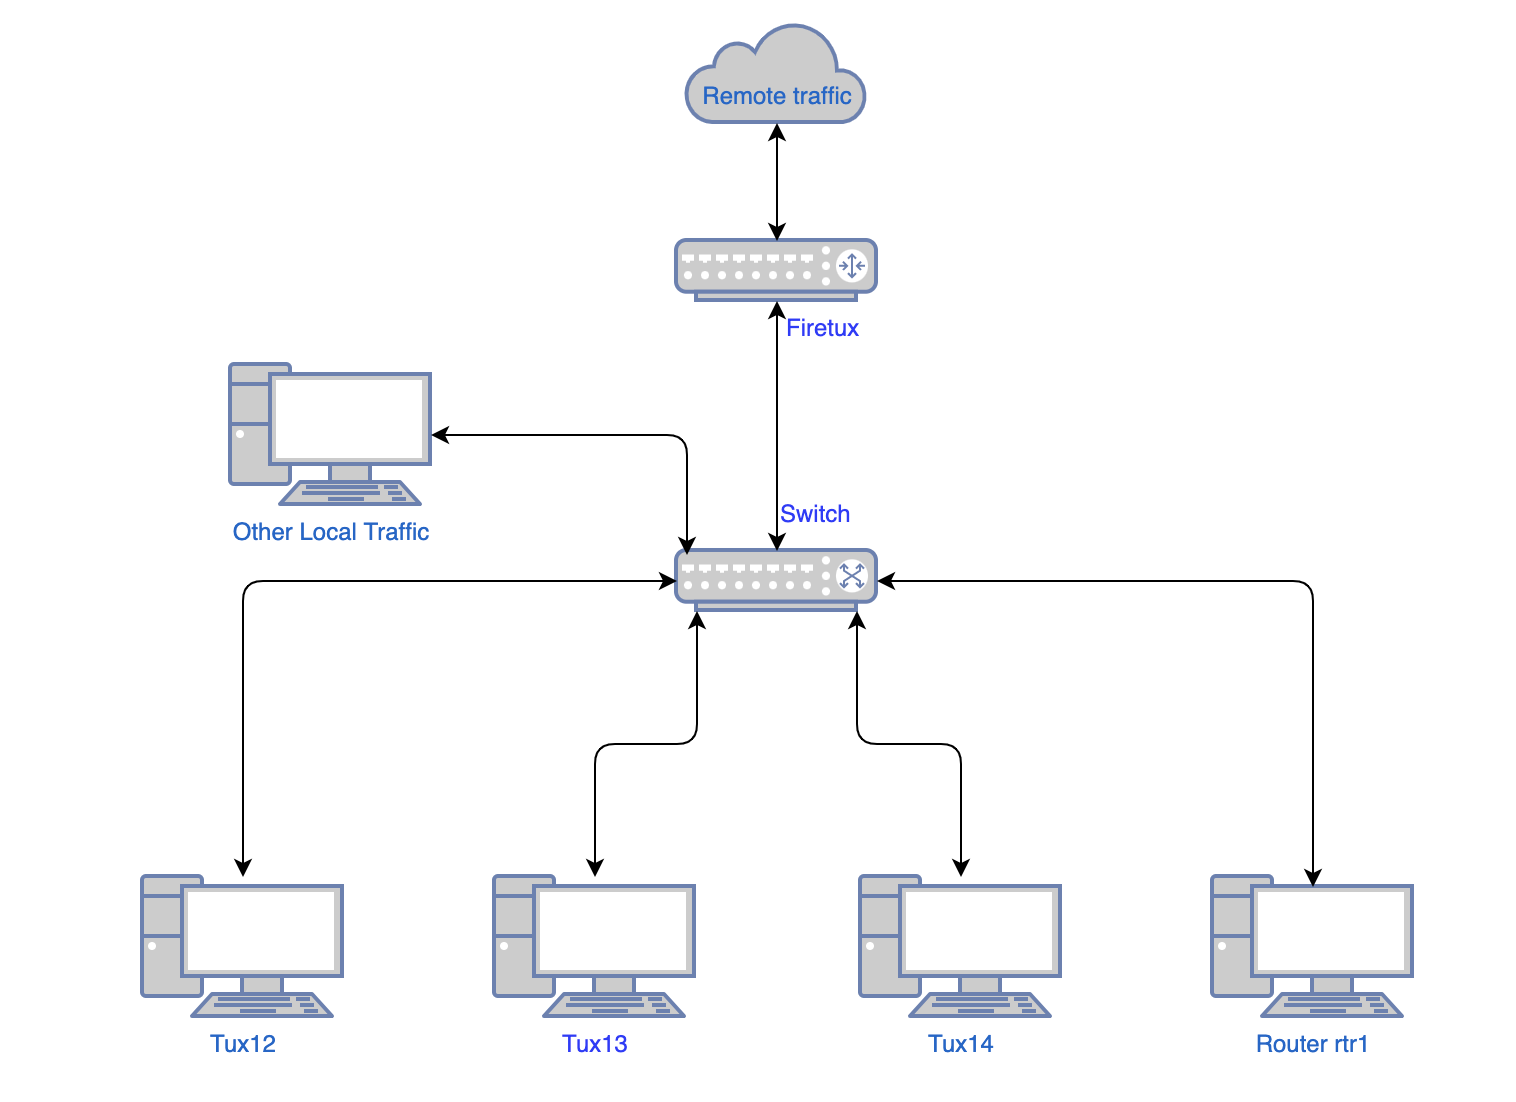
\includegraphics[width=.6\linewidth]{figs/setup/network.png}
    \caption{Configuração da rede neste trabalho}
    \label{fig:network}
\end{figure}

Devido à configuração da rede no laboratório, não é obrigatório que todo o tráfego passe pelo router de bancada (Fig \ref{fig:network}).

Em primeiro lugar, o \textbf{tráfego local} faz uso do \textbf{switch}, logo esse tráfego não será registado pelo MRTG dado que não passa pelo router de bancada.
Isto inclui todo o tráfego entre todos os \textit{tux}s da sala I321.

Em segundo lugar, o router de bancada faz parte da mesma rede local que os \textit{tux}s, ligados pelo switch ao router de sala \textbf{firetux}.
Deste modo, não é obrigatório que um acesso de um tux a um host externo passe pelo router de bancada.
Foi preciso então configurar os \textit{tux}s, de modo a que utilizassem o router de bancada como \textit{default gateway} para forçar o tráfego a ir por esse caminho.
O router de bancada por sua vez tem o router de sala como o seu \textit{default gateway} (Fig \ref{fig:traceroute_1}).
Isto só funciona para novos queries, dado que da segunda vez que fazemos um acesso, o algoritmo irá determinar automaticamente que o melhor caminho é diretamente pelo \textbf{firetux} e mais uma vez o tráfego não irá ser registado (Fig \ref{fig:traceroute_2}).

\begin{figure}
    \centering
    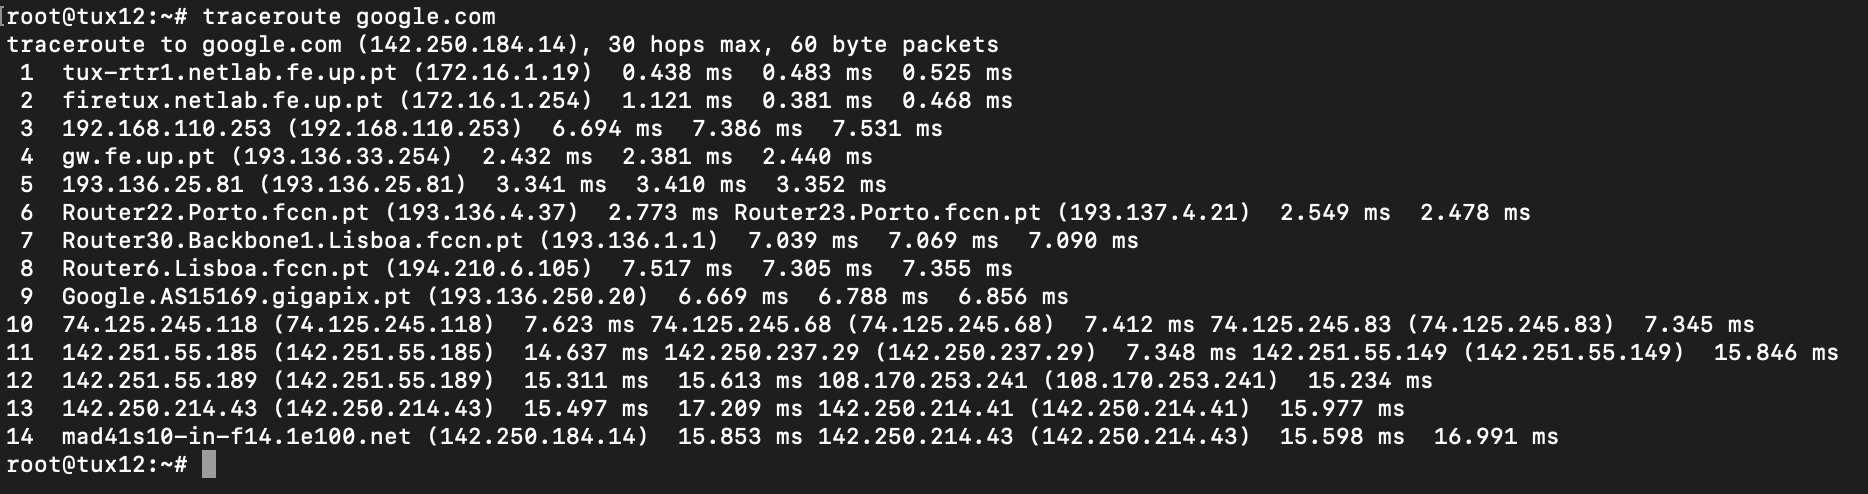
\includegraphics[width=.8\linewidth]{figs/setup/trace_1.png}
    \caption{Primeiro traceroute de google.com}
    \label{fig:traceroute_1}
\end{figure}

\begin{figure}
    \centering
    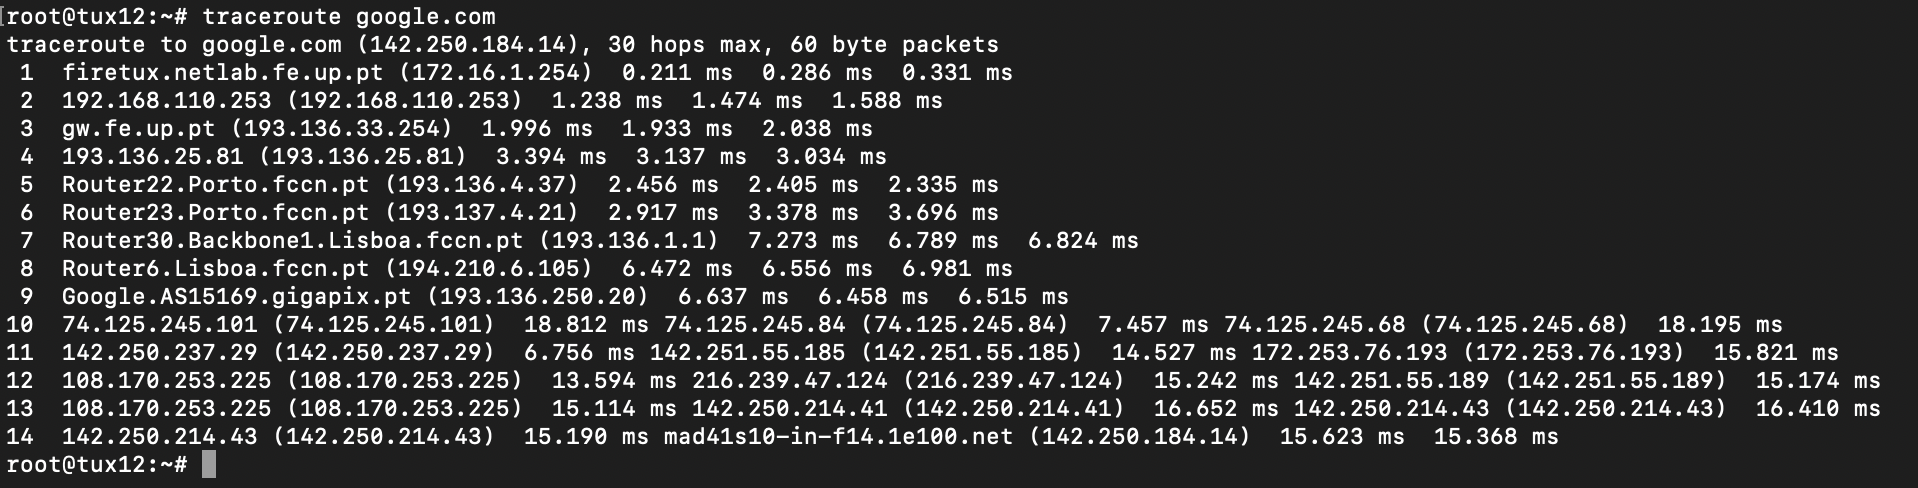
\includegraphics[width=.8\linewidth]{figs/setup/trace_2.png}
    \caption{Segundo traceroute de google.com}
    \label{fig:traceroute_2}
\end{figure}

Para voltar a forçar o caminho, é preciso apagar o routing cache, que é feito pelo próprio sistema periodicamente.

Em terceiro lugar, é preciso notar que o tráfego que vem de host externo \textbf{nunca} passa pelo router de bancada, a menos que seja direcionado para o mesmo.
Isto faz sentido dado que router de bancada não faz parte do caminho ótimo para os \textit{tux}.

Levanta-se então a nível do tráfego que nos é possível monitorizar. 
Todo o tráfego que é gerado no sentido \textit{Local->Remote} é monitorizado.
Tráfego \textit{Remote->Local / Local->Local} não é possível de observar.
Não podemos registar, por exemplo, acessos feitos ao nosso servidor FTP, ou emails enviados para o nosso servidor email.
A sincronização entre o NTP server e NTP client também não é analisado dado que é tráfego local.

Uma solução seria monitorizar o tráfego no switch, onde todo o tráfego passa obrigatoriamente. Teria por consequência ver-se no entanto também tráfego local de outras bancadas.

\subsection{Análise temporal}

O MRTG apresenta gráficos temporais do tráfego que passa pelo router, quer a entrar, quer a sair.
Devido ao período de tempo em que este esteve a monitorizar, só faz sentido apresentar o gráfico diário e semanal (Fig \ref{fig:mrtg_main}).

\begin{figure}
    \centering
    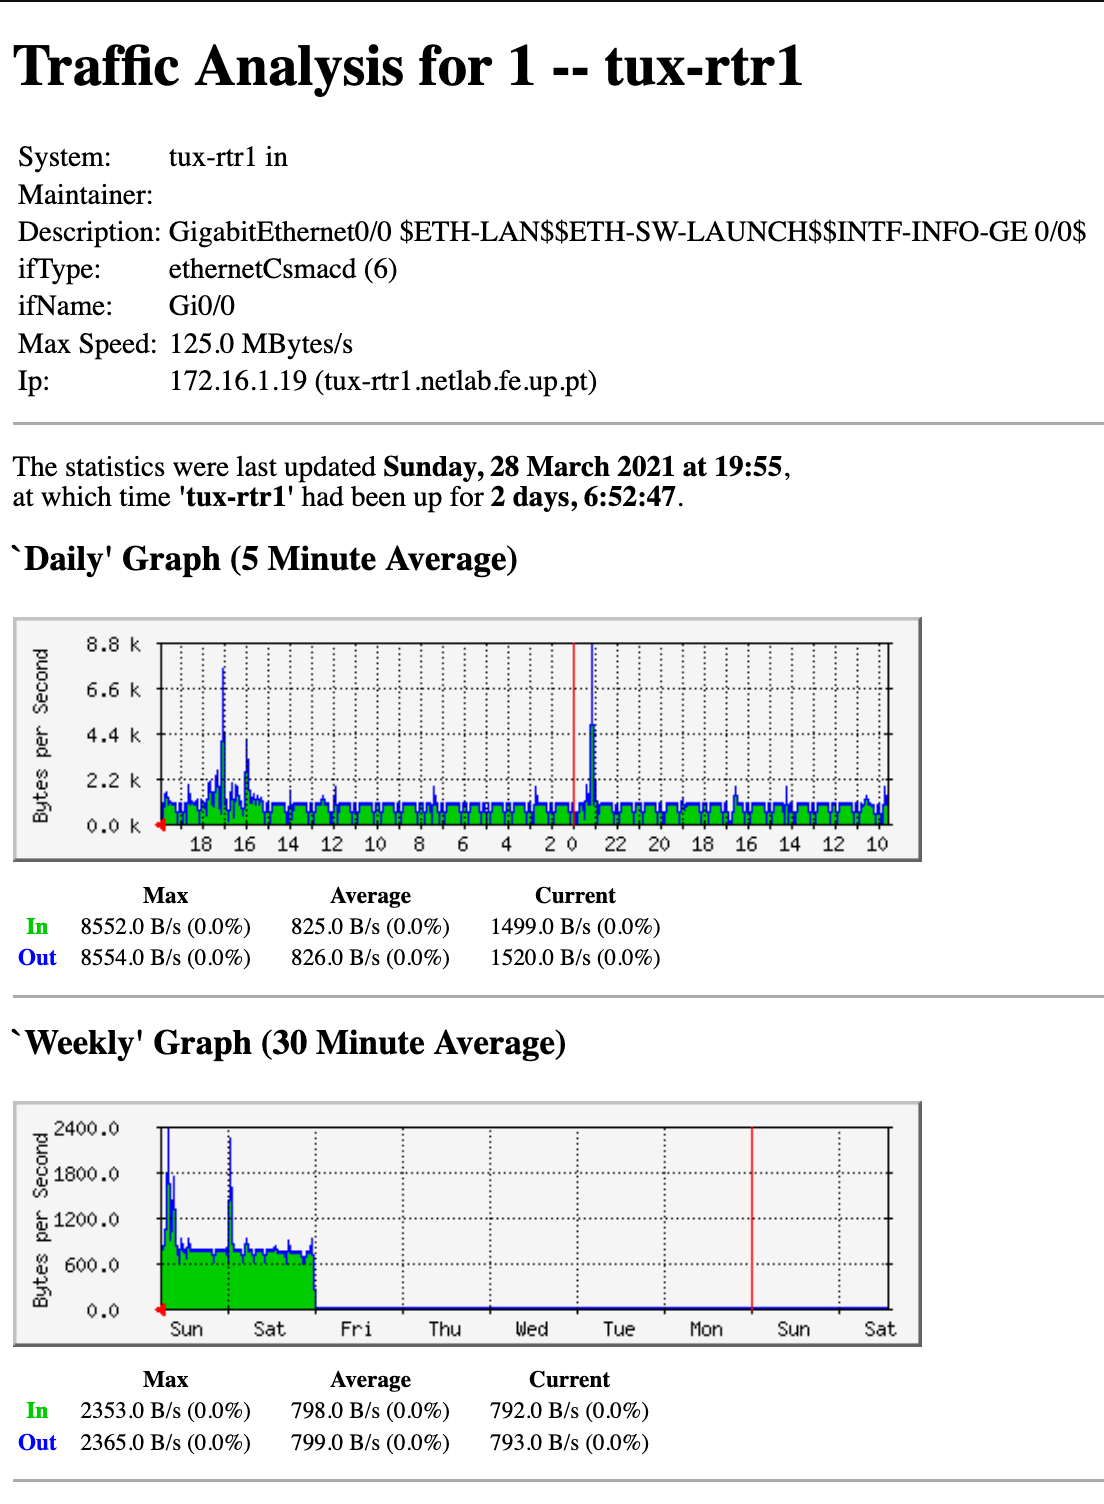
\includegraphics[width=.6\linewidth]{figs/setup/mrtg.png}
    \caption{Gráficos temporais do tráfego no router MRTG}
    \label{fig:mrtg_main}
\end{figure}

Como se pode observar, o gráfico é constante e apresenta um padrão a nível de picos que está relacionado com a temporização dos cronjobs.
Estes cronjobs fazem diferentes tarefas como enviar mails, fazer "digs" no DNS e aceder a servidores HTTP.
Os picos maiores devem-se a testes que estavam ser executados durante a configuração o sistema, como, por exemplo, pelo envio de muitos emails num curto espaço de tempo.

Constatamos também que o tráfego que entra é praticamos igual ao tráfego que sai. 
Isto deve-se ao facto de muito pouco tráfego ser destinado ao próprio router, funcionando este apenas como uma \textit{gate}.

\section{NTOP}

\subsection{Configuração}

O \textbf{NTOP} é uma ferramenta de monitorização de tráfico. Oferece uma versão comunitária grátis, assim como versões profissionais de subscrição.

O NTOP funciona escutando o tráfego num adaptador de rede, i.e., interface. No nosso caso, é utilizada a interface \textit{eth0}. É de notar que o NTOP consegue monitorizar várias interfaces ao mesmo tempo.
Desse modo, este foi configurado para escutar essa interface \cite{ntop}. A web-app do NTOP é acedida através do link \verb|172.16.1.12:3000| e depois é efetuado o login com os dados configurados.

\subsection{Análise global}

Dentro da web-app do NTOP, após selecionar a interface desejada, é-nos apresentada uma página inicial onde se pode observar resumo do tráfego nessa interface: (Fig \ref{fig:ntop_main})
\begin{itemize}
    \item Monitorização do tráfego em tempo real no canto superior esquerdo
    \item Tipo de tráfego, com 86\% a ser \textit{Local->Remote}.
    \item Total de tráfego registado pelo NTOP, com 205 MB enviado e 41.6 MB recebidos. Dado que estão a ser realizados acessos FTP externos, ocorre um aumento considerável do total de MB enviados pelo servidor.
\end{itemize}

\begin{figure}
    \centering
    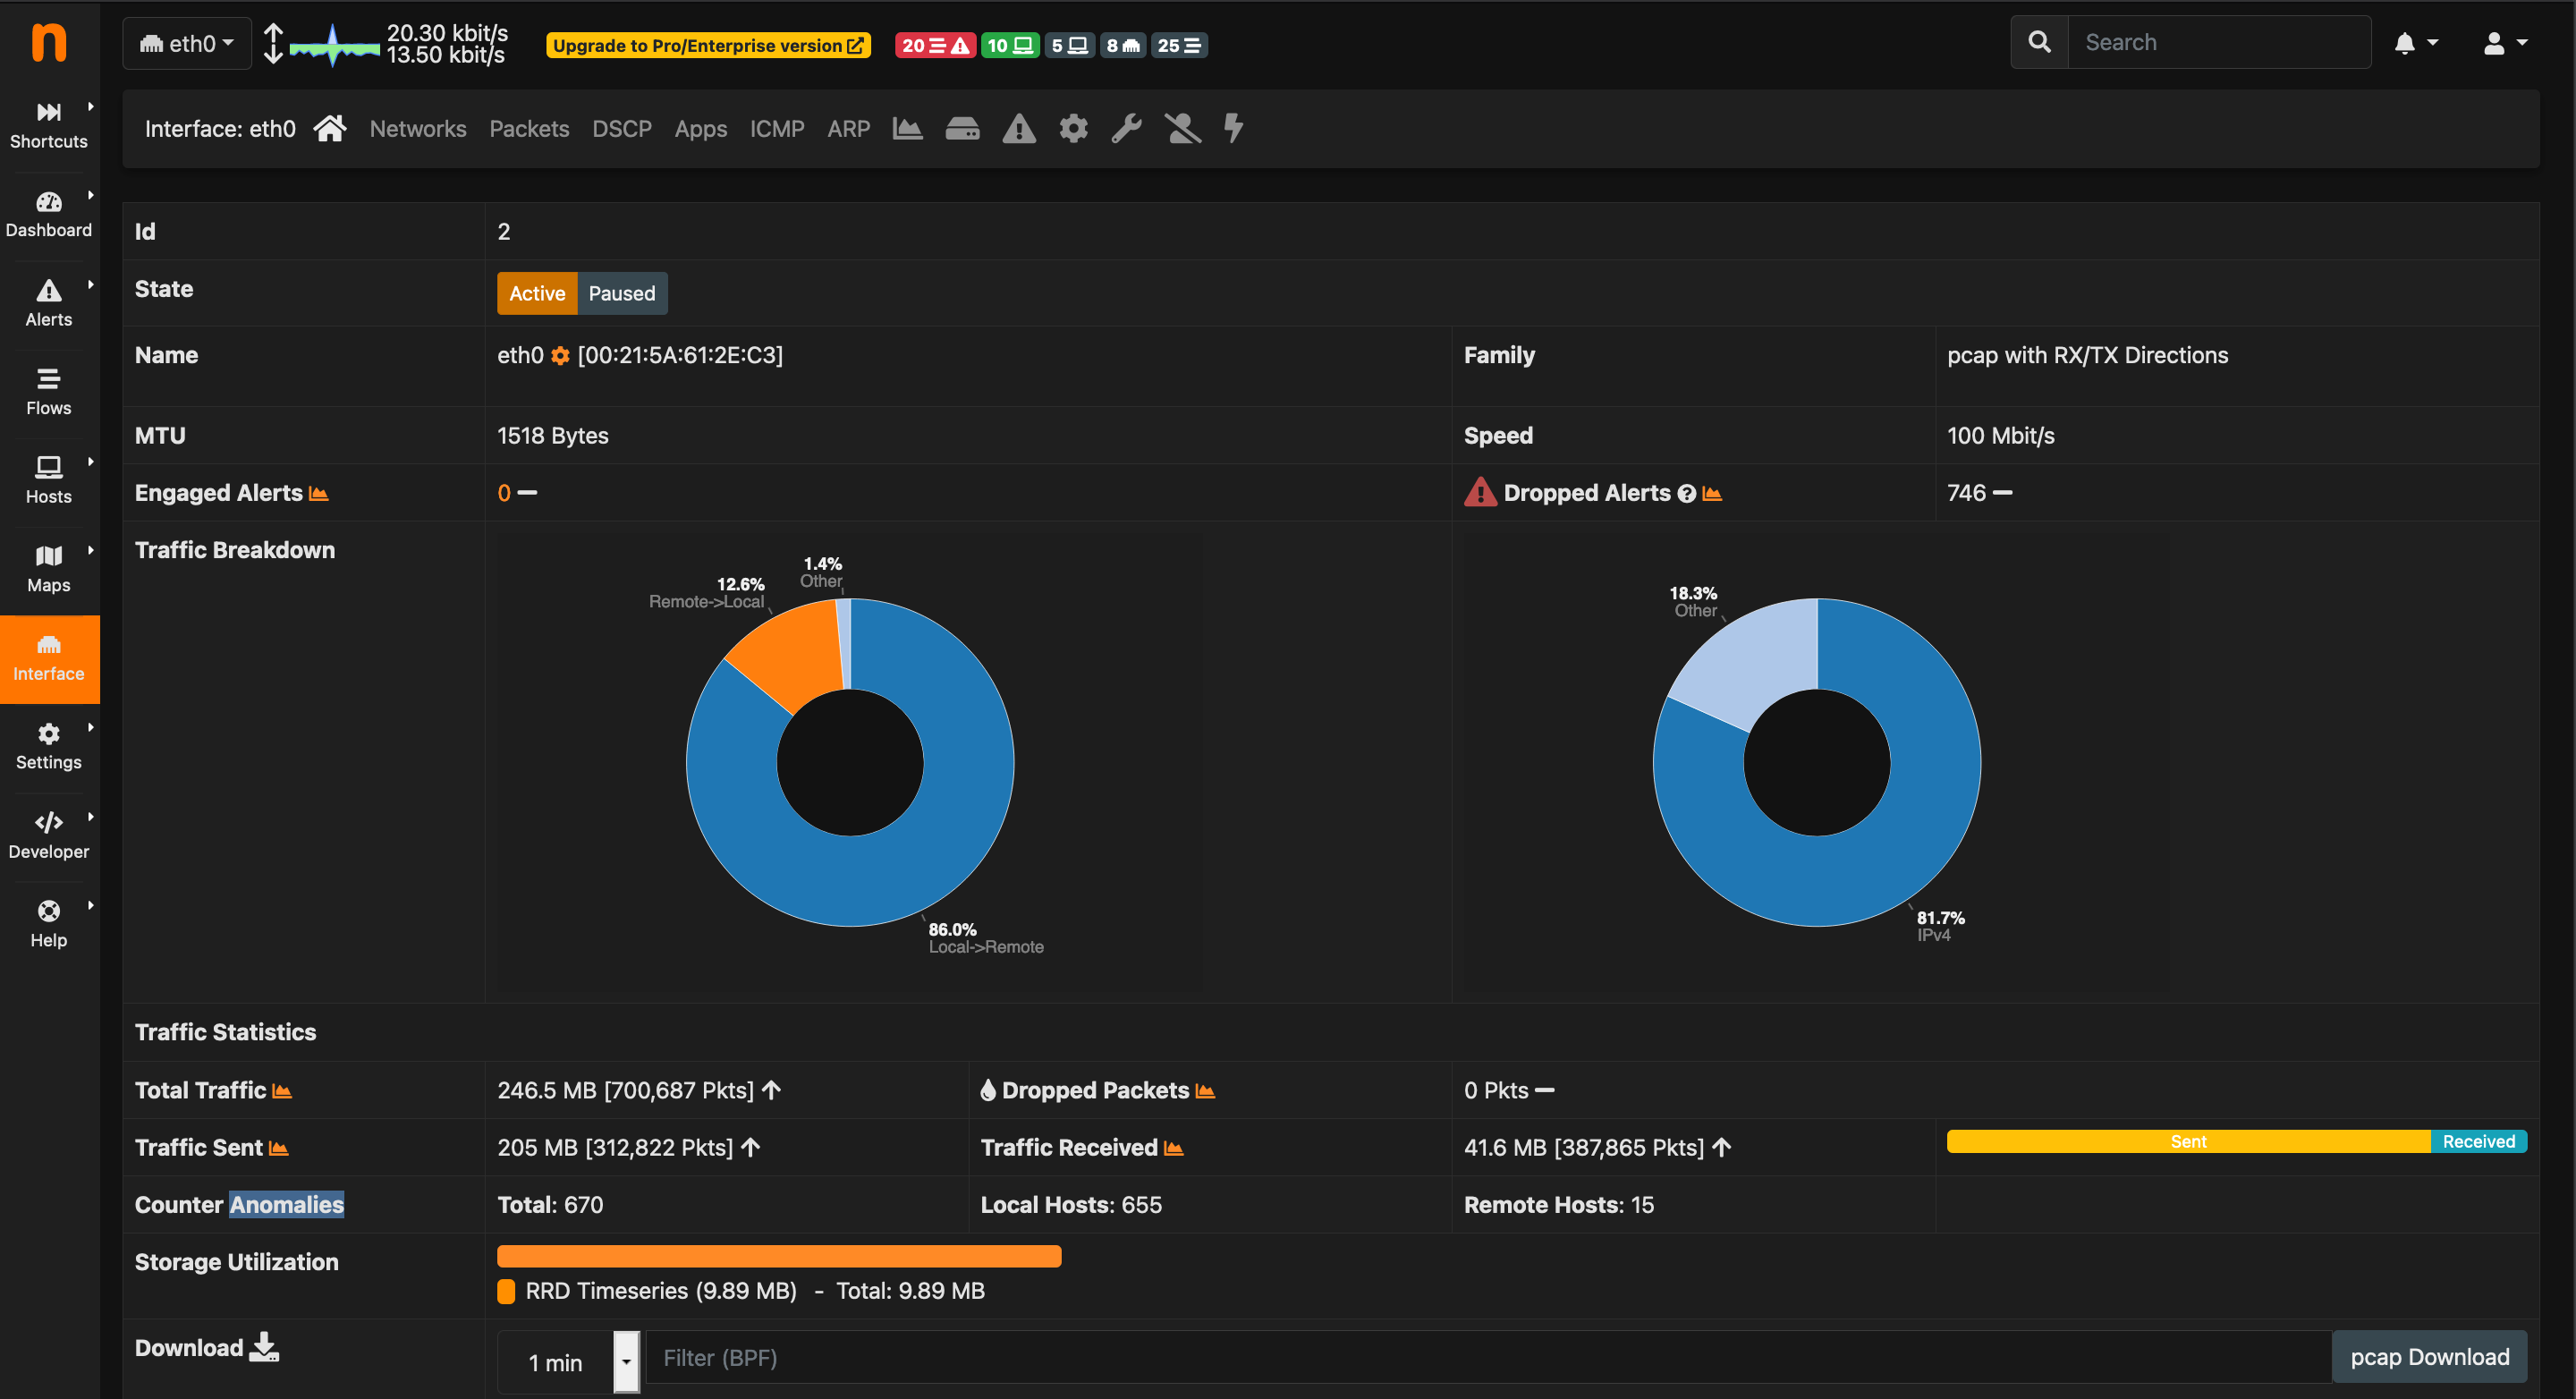
\includegraphics[width=.8\linewidth]{figs/setup/ntop_main.png}
    \caption{Main page da interface eth0}
    \label{fig:ntop_main}
\end{figure}

\subsection{Análise por tipologia}

Na tab "Apps", são apresentados 4 piecharts contendo a distribuição do tráfego por tipologia.
É apresentada uma avaliação total, assim como uma monitorização em tempo real (Fig \ref{fig:apps_charts}).

O \textit{FTP Data} corresponde a 52.4\% do tráfego, com o NTOP a representar 28.2\%.
Isto deve-se ao facto do NTOP gerar informação em realtime, que obriga a atualização constante da informação, gerando mais tráfego.
No momento em que foi tirado o print, não estava a ser detetado tráfego significativo de outros serviços, por isso o NTOP representa a maior fatia.

\begin{figure}
    \centering
    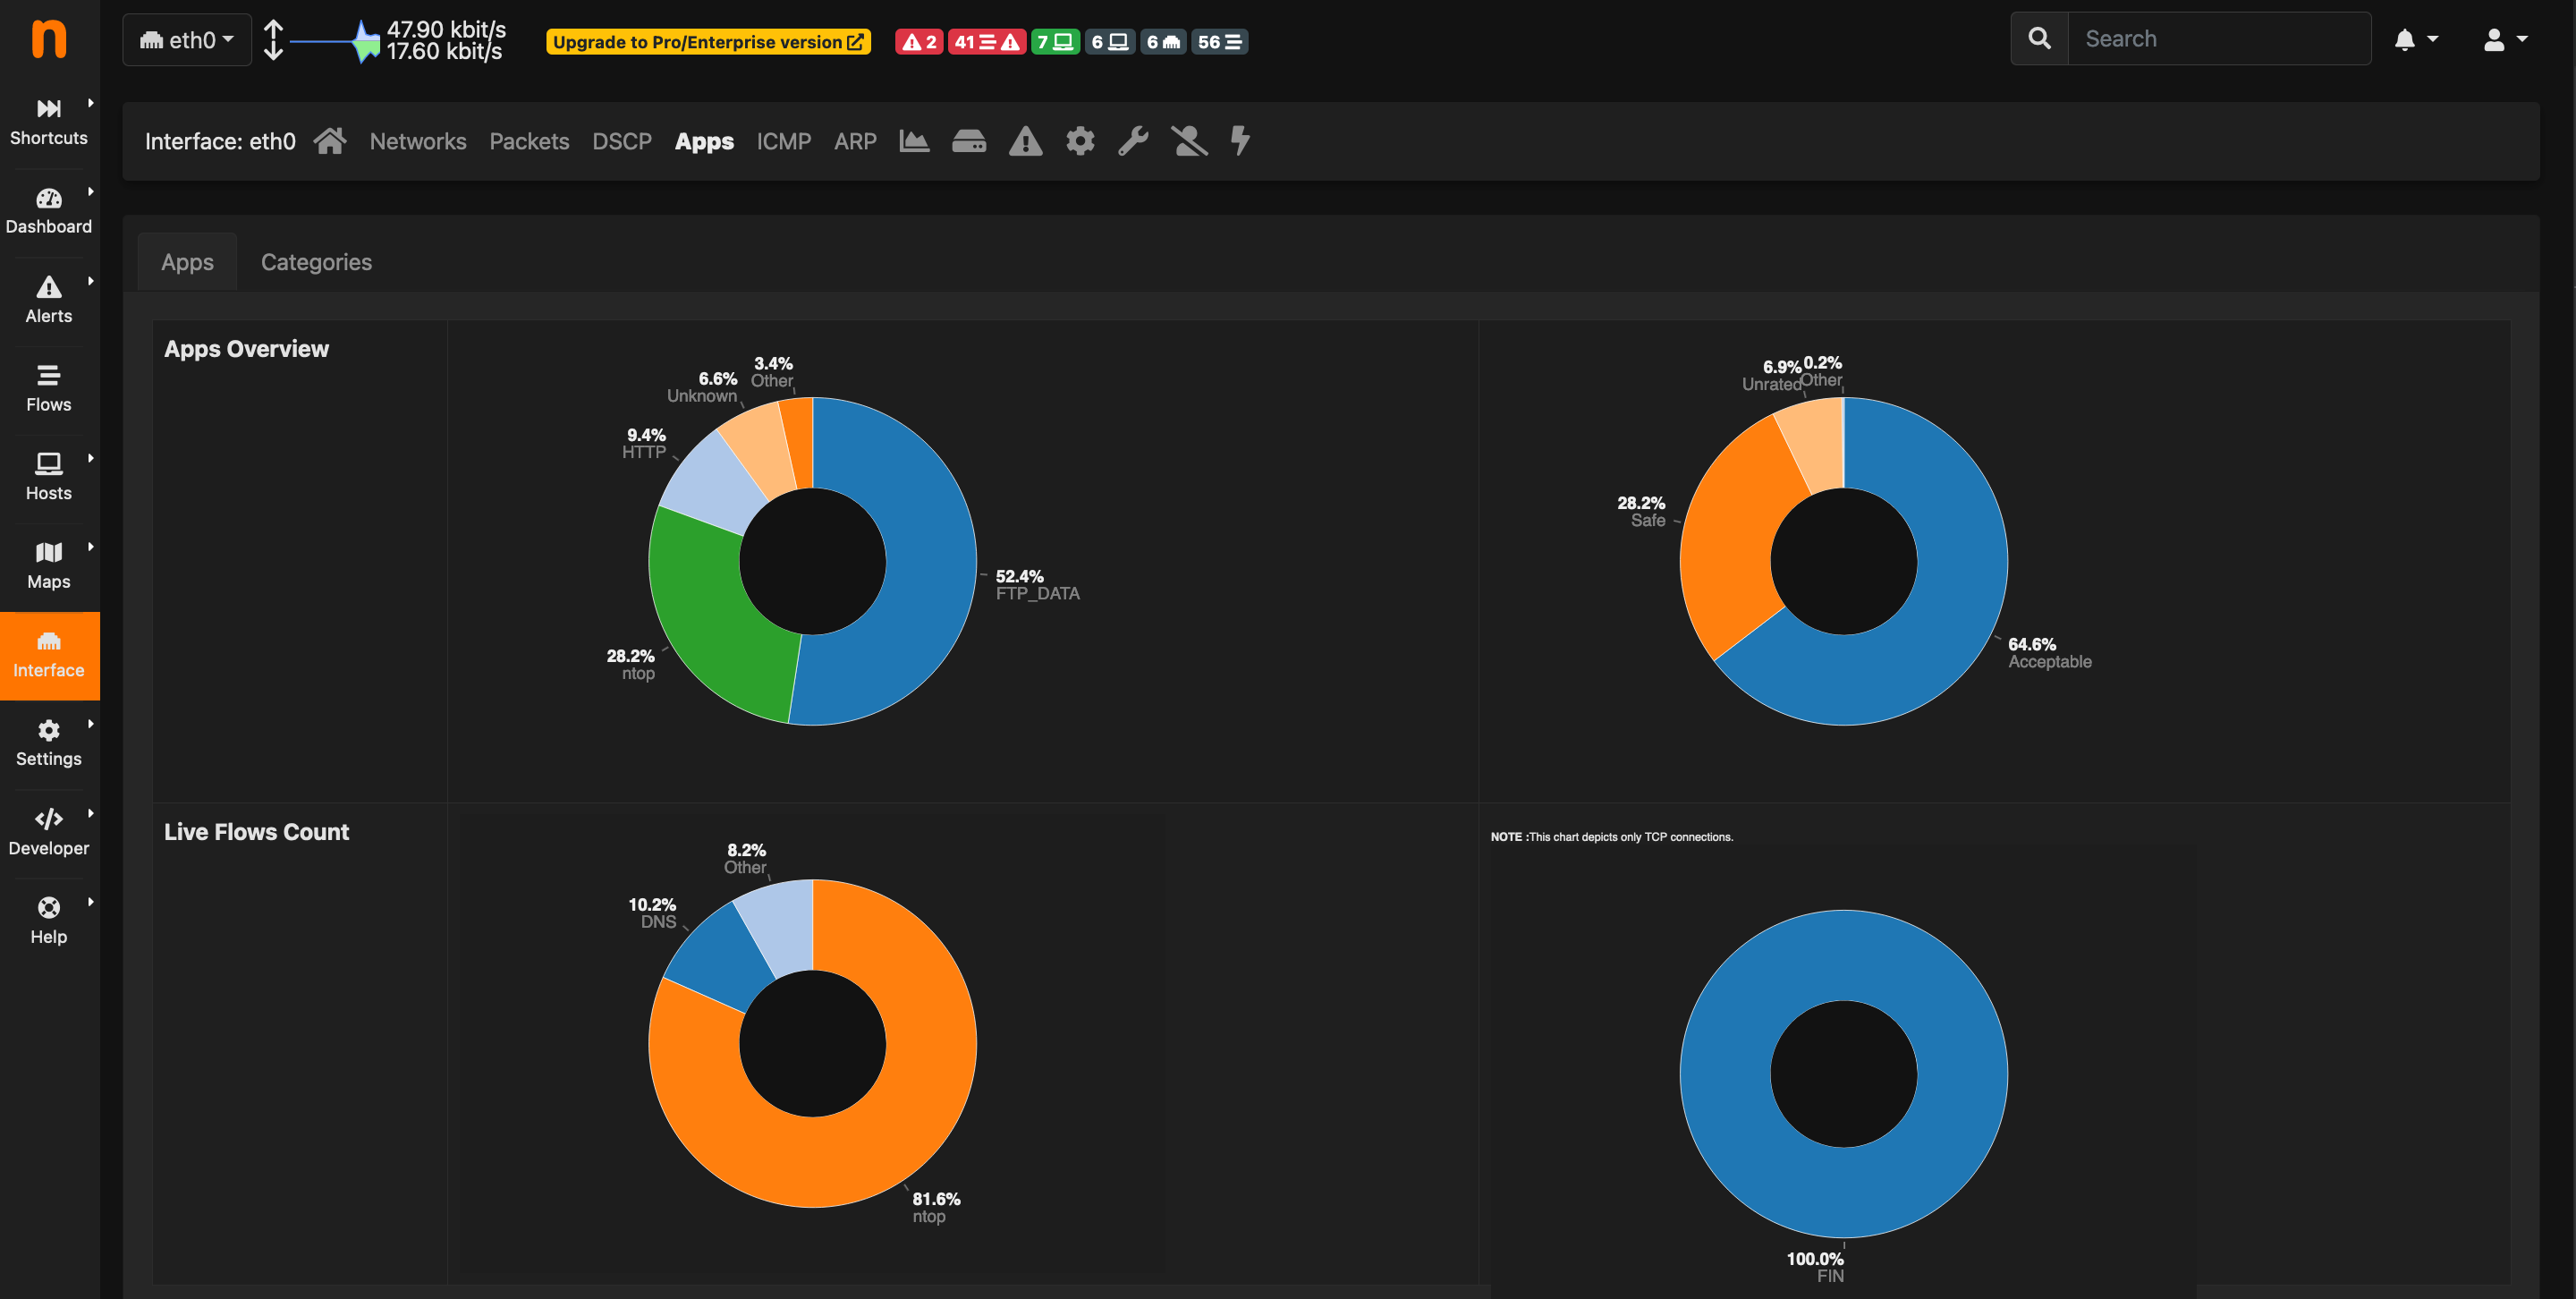
\includegraphics[width=.8\linewidth]{figs/setup/apps_charts.png}
    \caption{Piecharts da distribuição do tráfego por tipologia}
    \label{fig:apps_charts}
\end{figure}

Conseguimos também ver a distribuição total do tráfego em valores absolutos, onde podemos observar,
por exemplo, que o tráfego FTP representa a maior fatia de tráfego na interface (Fig \ref{fig:apps_table}).
Conseguimos também observar tráfego dos outros serviços instalados, nomeadamente DNS, HTTP, NTP e SMTP (Simple Mail Transfer Protocol).
O FTP estava a ser acedido para fazer download de um ficheiro de 250 Kb, pelo que gera mais tráfego.
O email por outro lado, era pequeno, pelo que gera menos tráfego.
Outros serviços são também detetados.


\begin{figure}
    \centering
    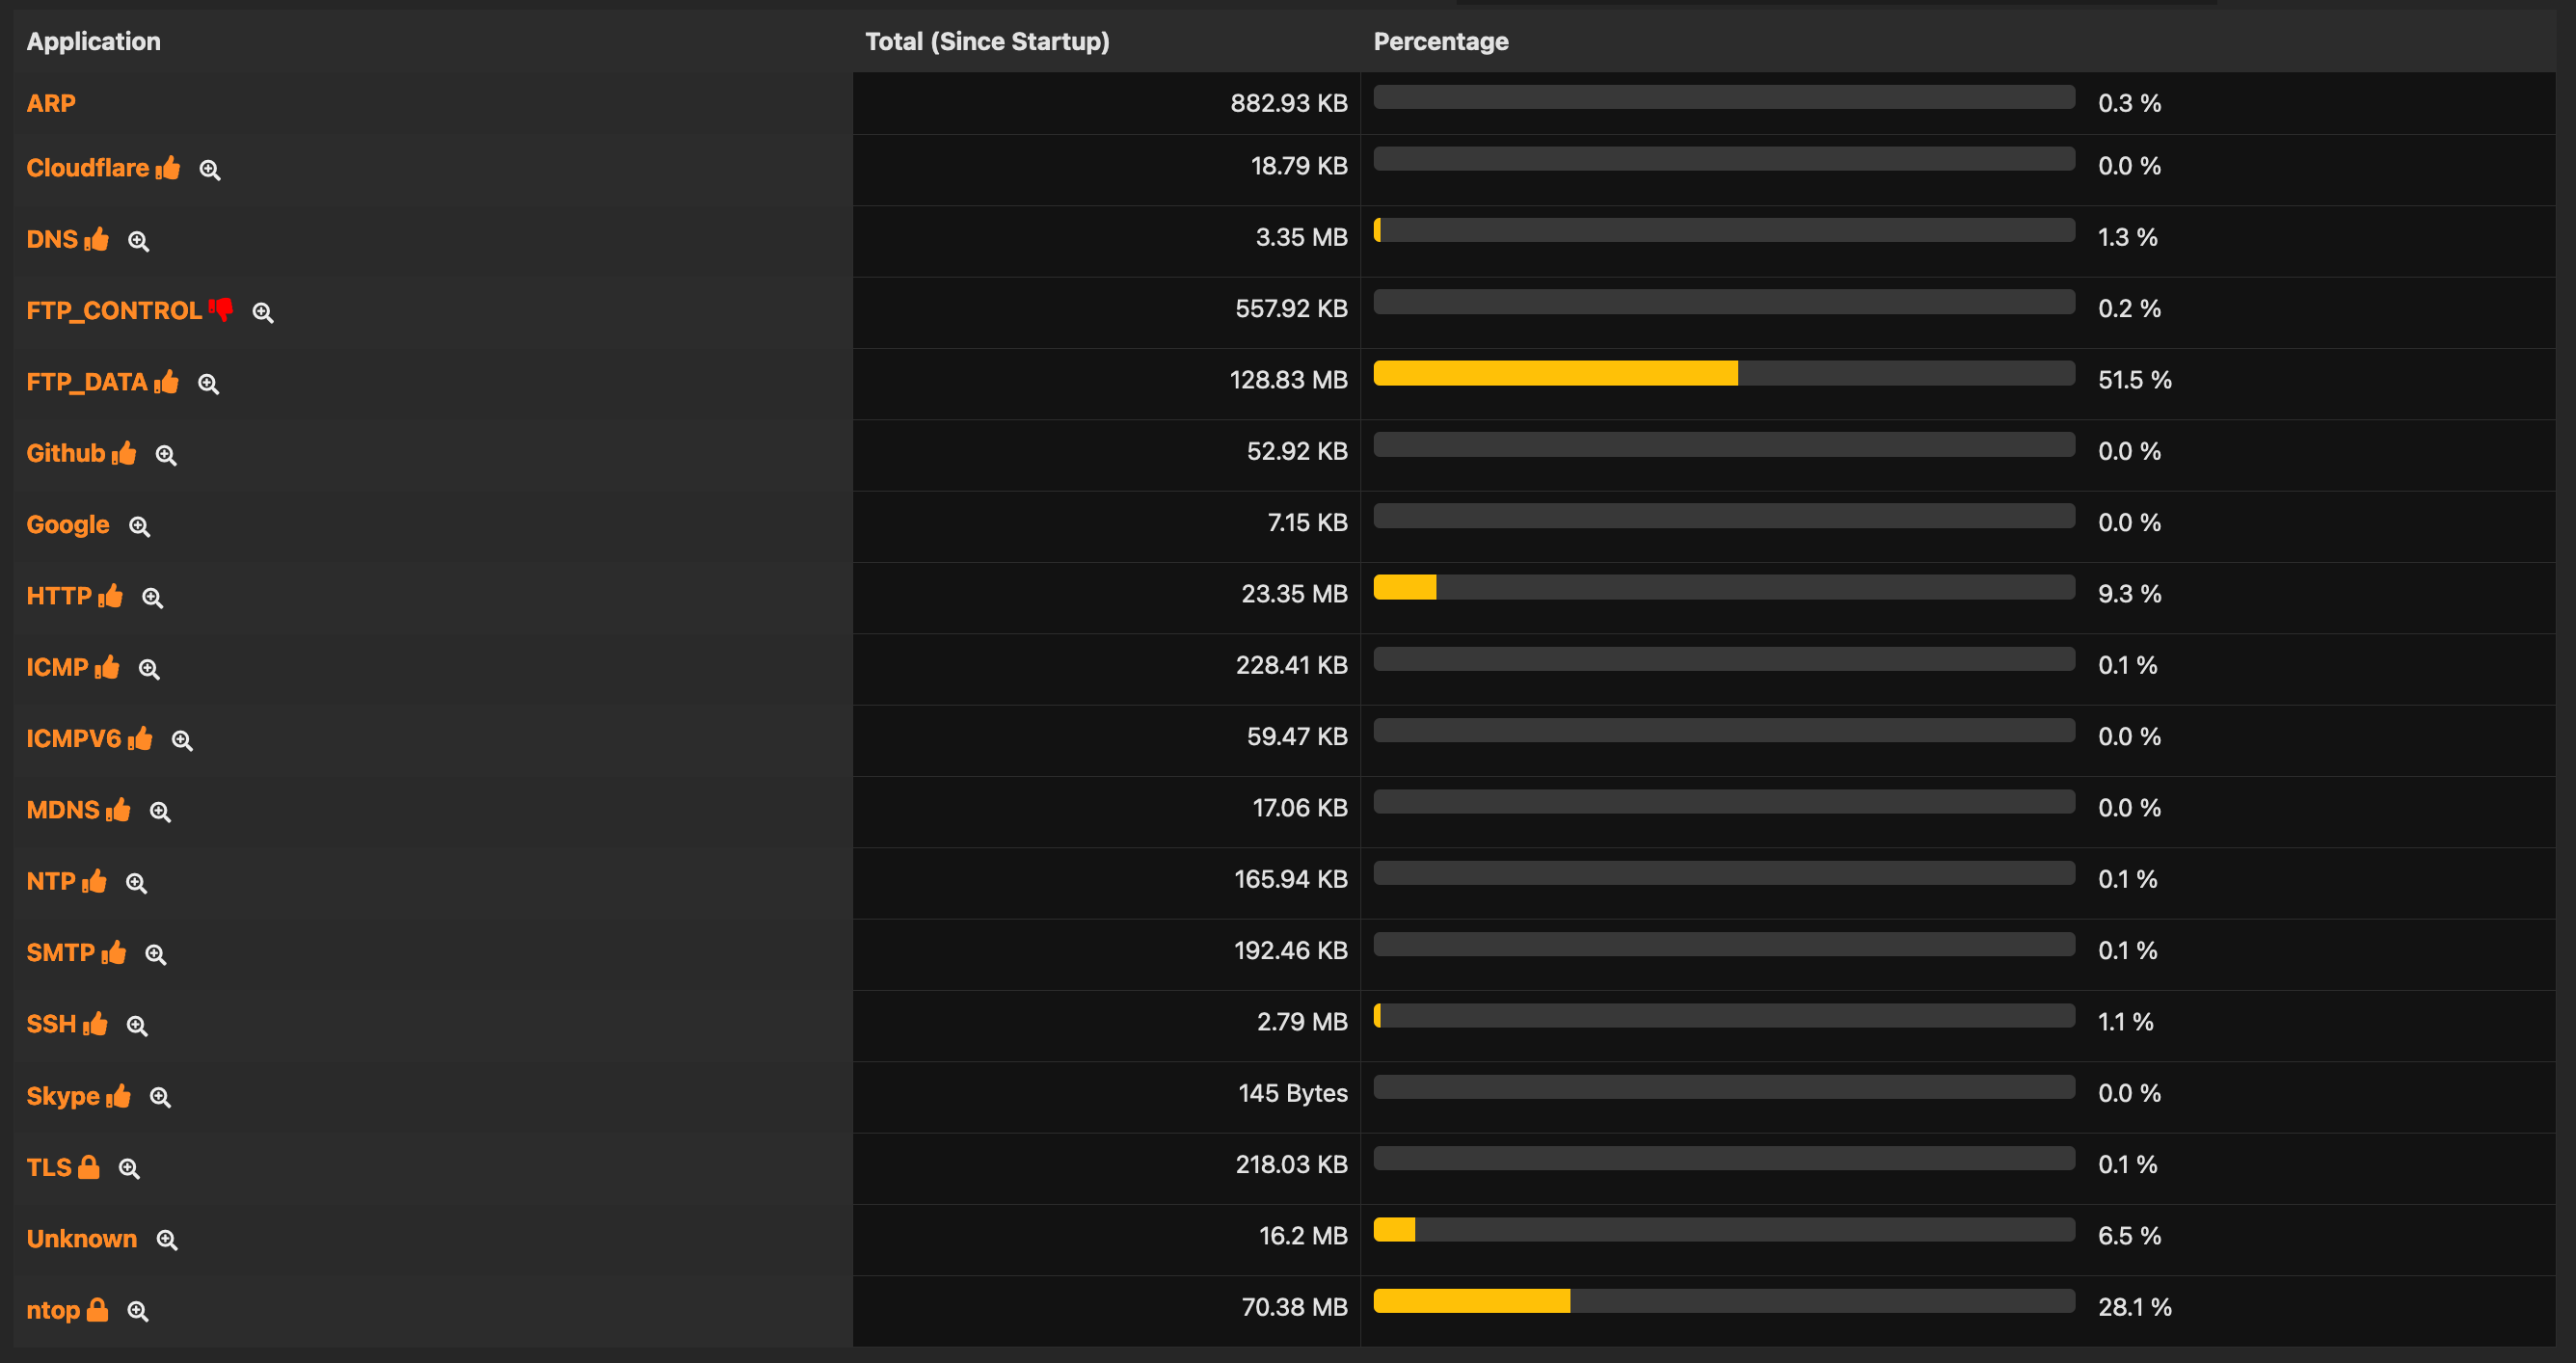
\includegraphics[width=.8\linewidth]{figs/setup/apps_tables.png}
    \caption{Distribuição do tráfego por tipologia}
    \label{fig:apps_table}
\end{figure}

\subsection{Análise temporal}

Tal como o MRTG, o NTOP também apresenta gráficos com a distribuição do tráfego a nível temporal.
Podemos observar diferentes intervalos temporais, como por exemplo, o horário (Fig \ref{fig:hourly}).
Podemos constatar neste gráfico vários picos periódicos de tráfego.
Estes correspondem, mais uma vez, aos pedidos FTP que geram muito mais tráfego que os restantes serviços.

\begin{figure}
    \centering
    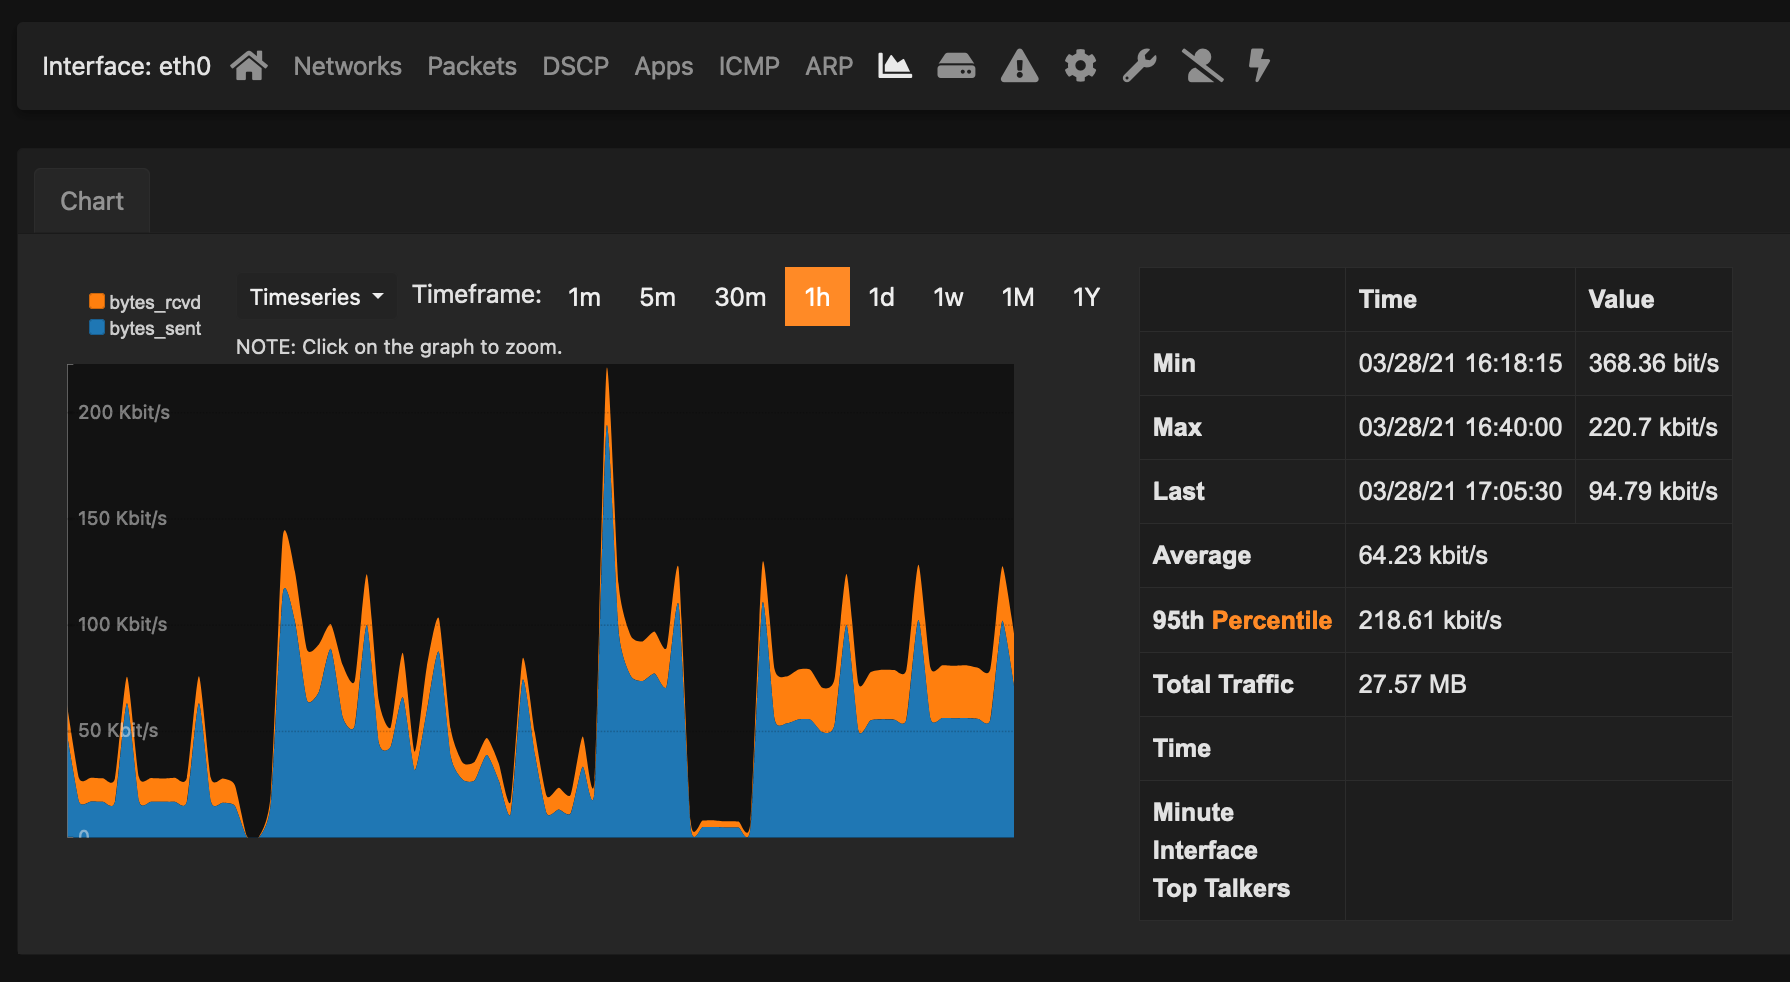
\includegraphics[width=.8\linewidth]{figs/setup/hourly.png}
    \caption{Análise horária do tráfego}
    \label{fig:hourly}
\end{figure}

\subsection{Análise dos Hosts}

O NTOP apresenta também uma lista de hosts que utilizaram a interface para enviar/receber tráfego (Fig \ref{fig:hosts}).
Esta lista é dinâmica e apresenta apenas os hosts ativos recentemente, mas é possível fazer uma pesquisa por qualquer host que tenha utilizado a interface.
Podemos constatar que o \textit{tux12} (172.16.1.12) gerou a maior parte do tráfego (243.74 MB).
Isto faz sentido dado que foi neste \textit{tux} que se instalaram todos os serviços.

\begin{figure}
    \centering
    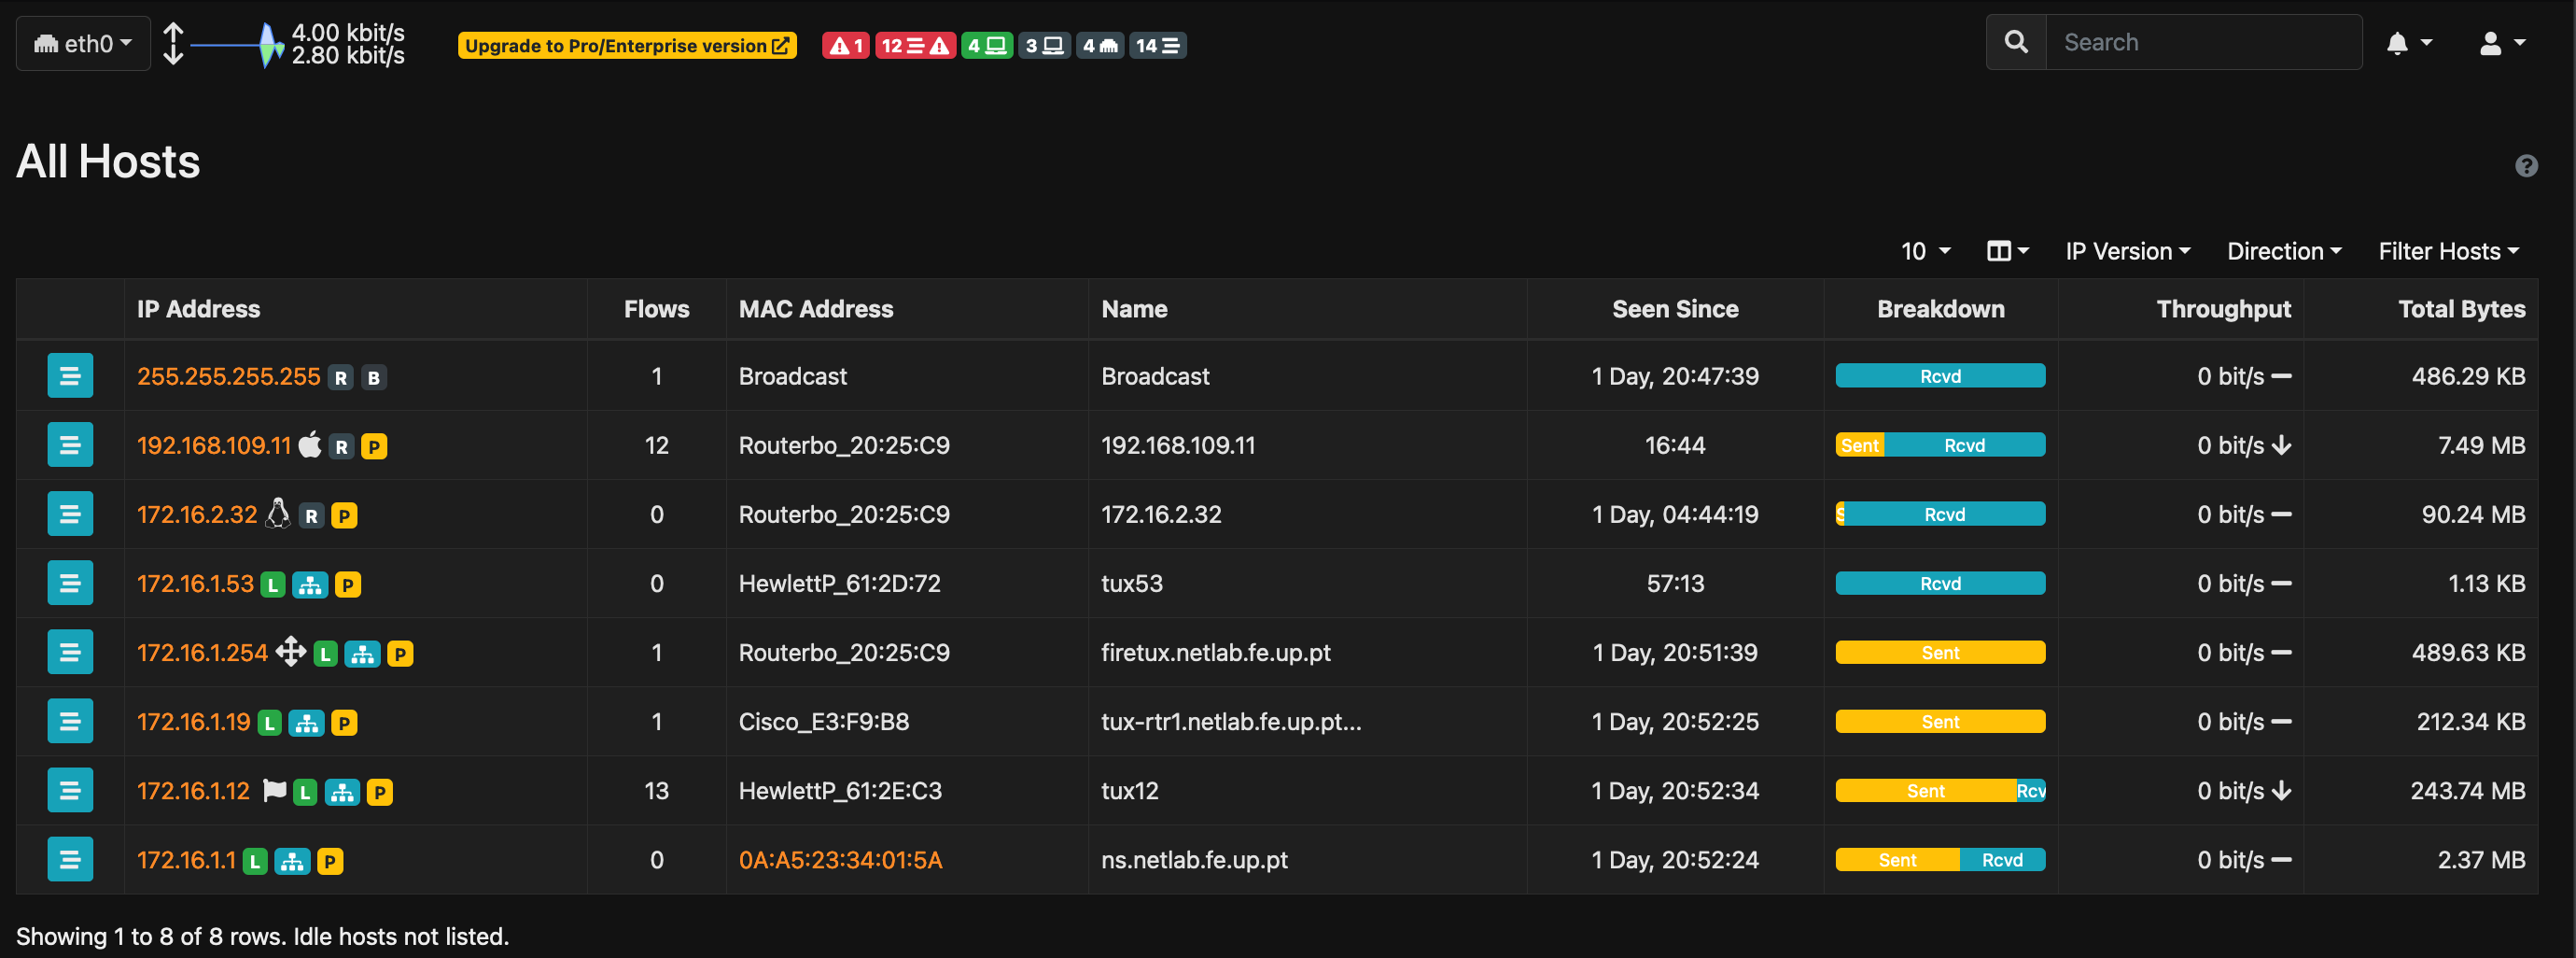
\includegraphics[width=.8\linewidth]{figs/setup/hosts.png}
    \caption{Lista dinâmica de hosts ativos}
    \label{fig:hosts}
\end{figure}

Também é possível fazer o mesmo tipos de análises que foram feitas para a interface, como a distribuição por tipologia e a distribuição temporal (Fig \ref{fig:hosts_apps}).

\begin{figure}
    \centering
    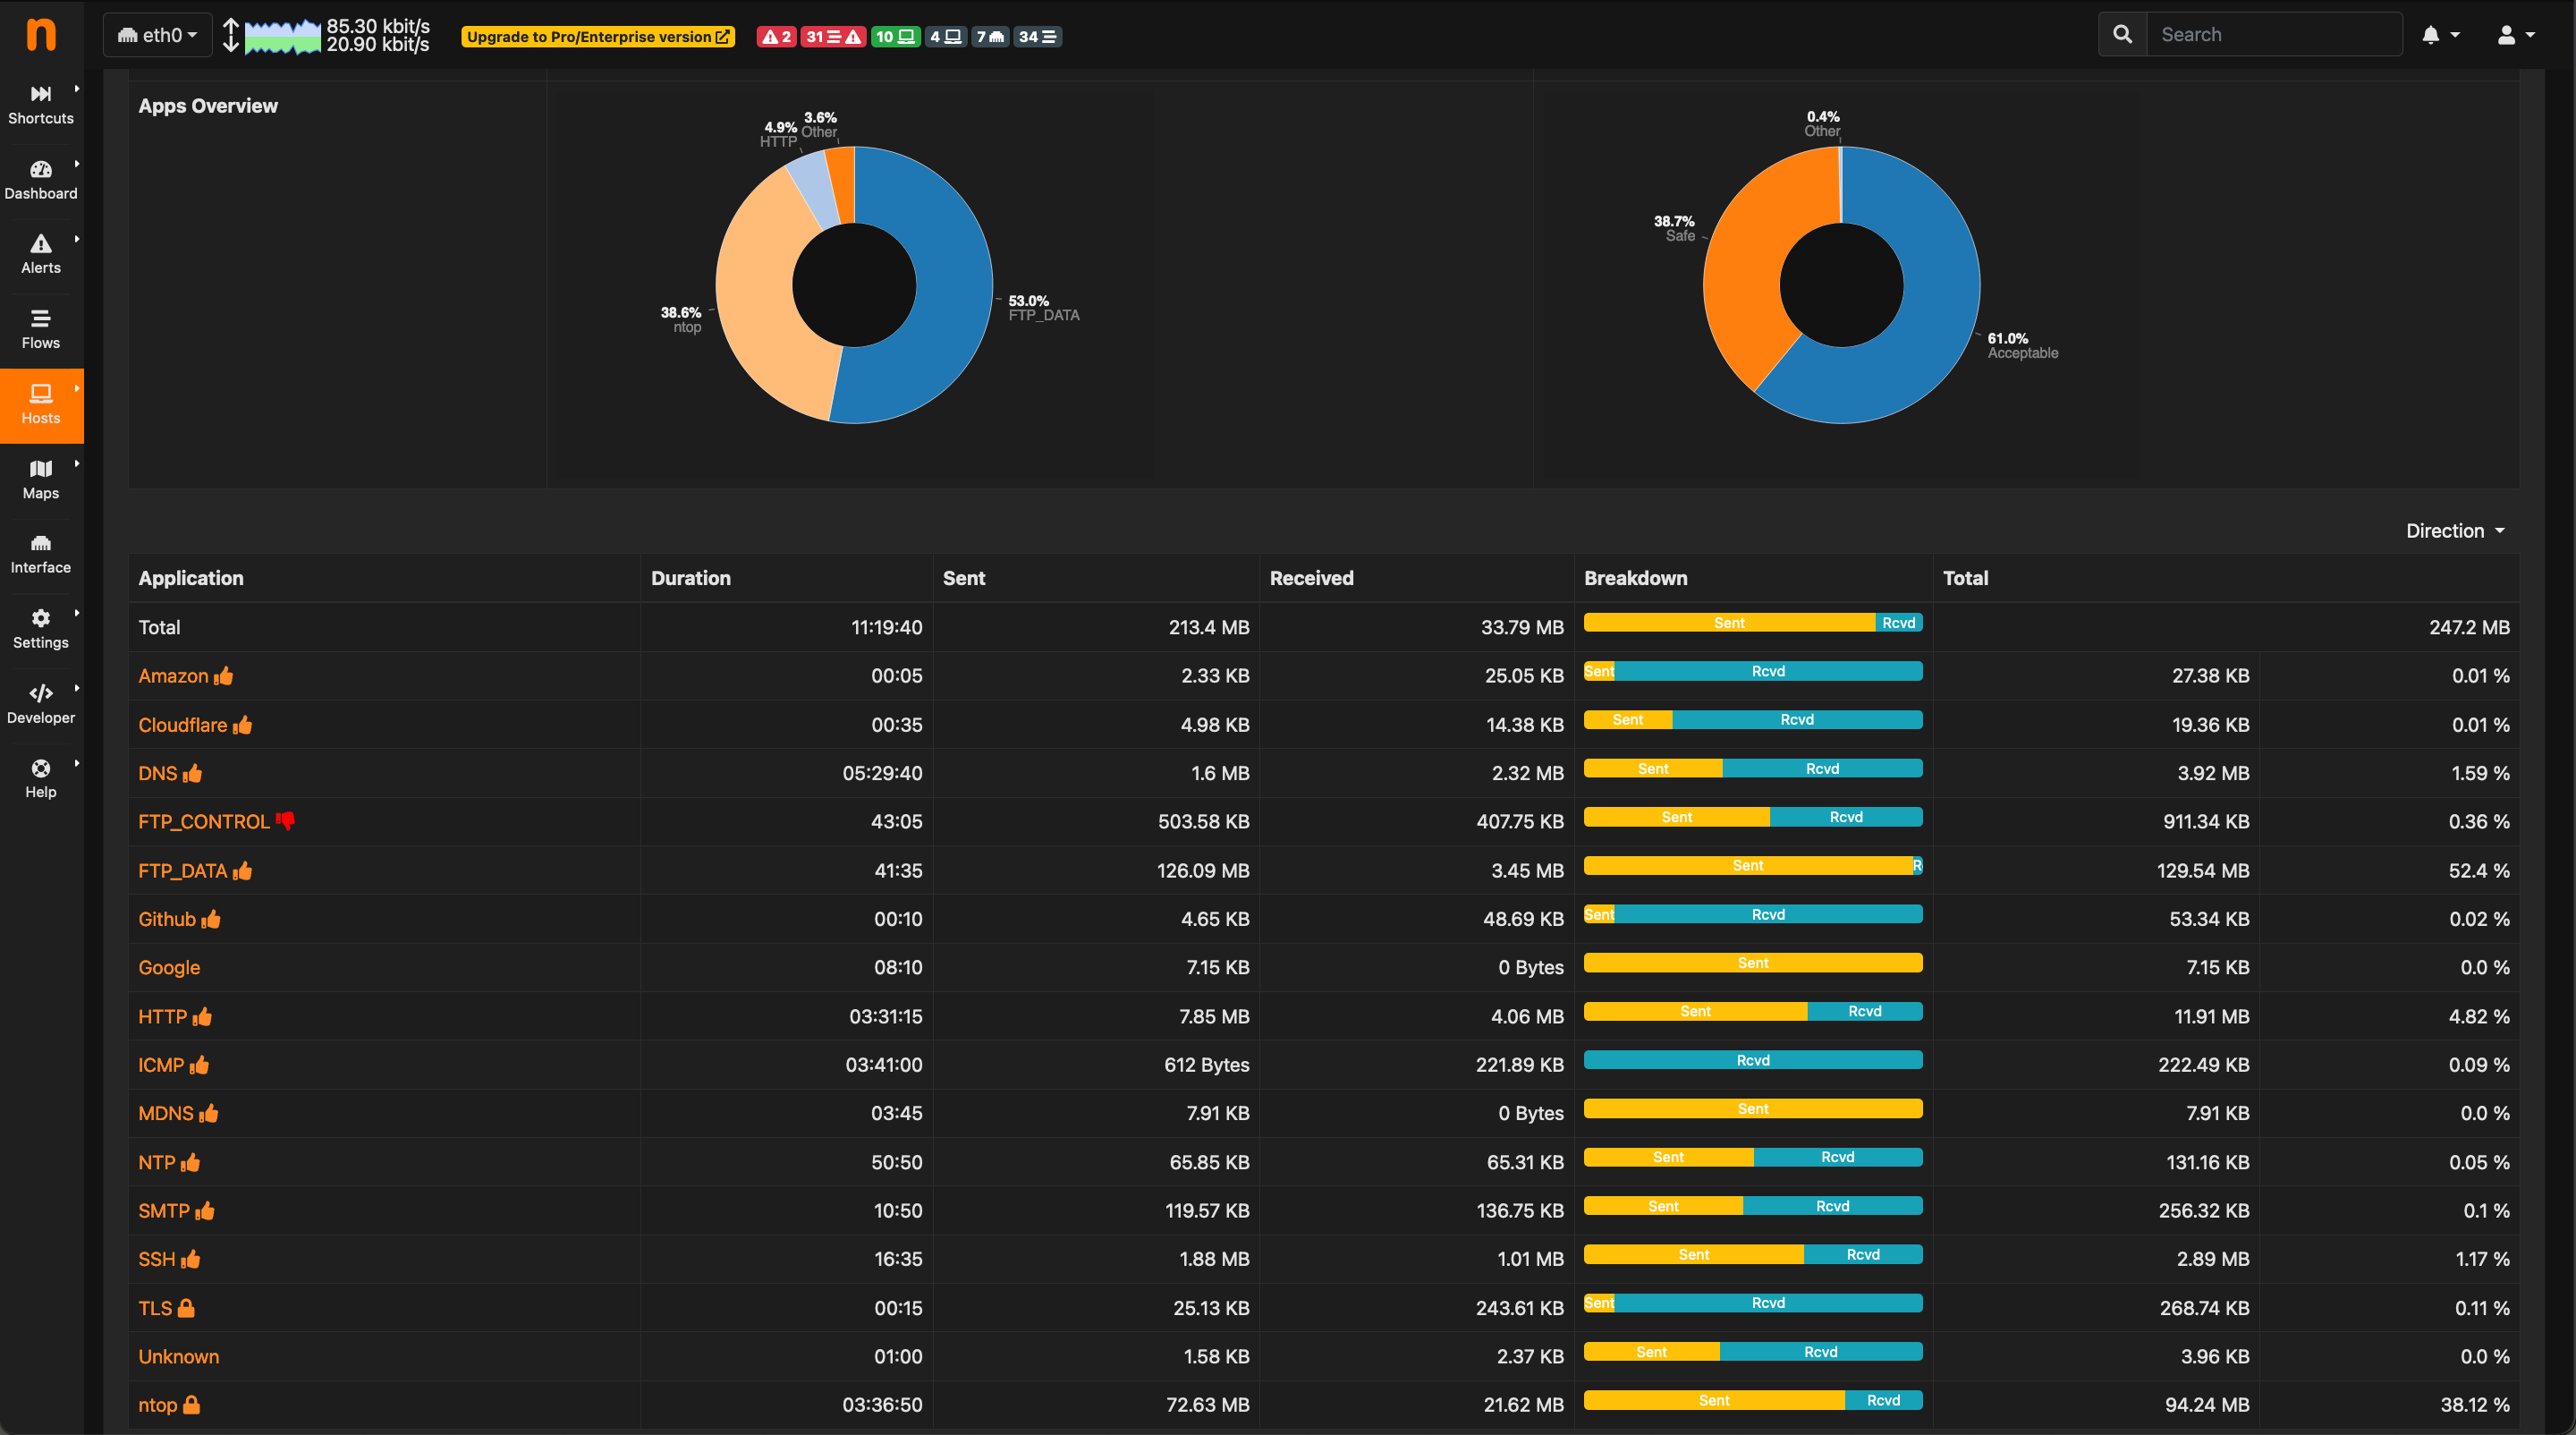
\includegraphics[width=.8\linewidth]{figs/setup/host_apps.png}
    \caption{Distribuição do tráfego por tipologia no tux12}
    \label{fig:hosts_apps}
\end{figure}

\subsection{Análise dos recursos do Sistema}

Além da análise do tráfego da interface, o NTOP apresenta também os recursos do sistema onde está instalado e o seu nível de utilização (Fig \ref{fig:system}).
Podemos observar gráficos de utilização do CPU do sistema para avaliar possíveis \textit{bottlenecks} a nível do hardware.
No nosso caso, os serviços instalados e a sua utilização não representam uma carga de utilização suficientemente grande para esta ferramenta ser útil neste projeto.

\begin{figure}
    \centering
    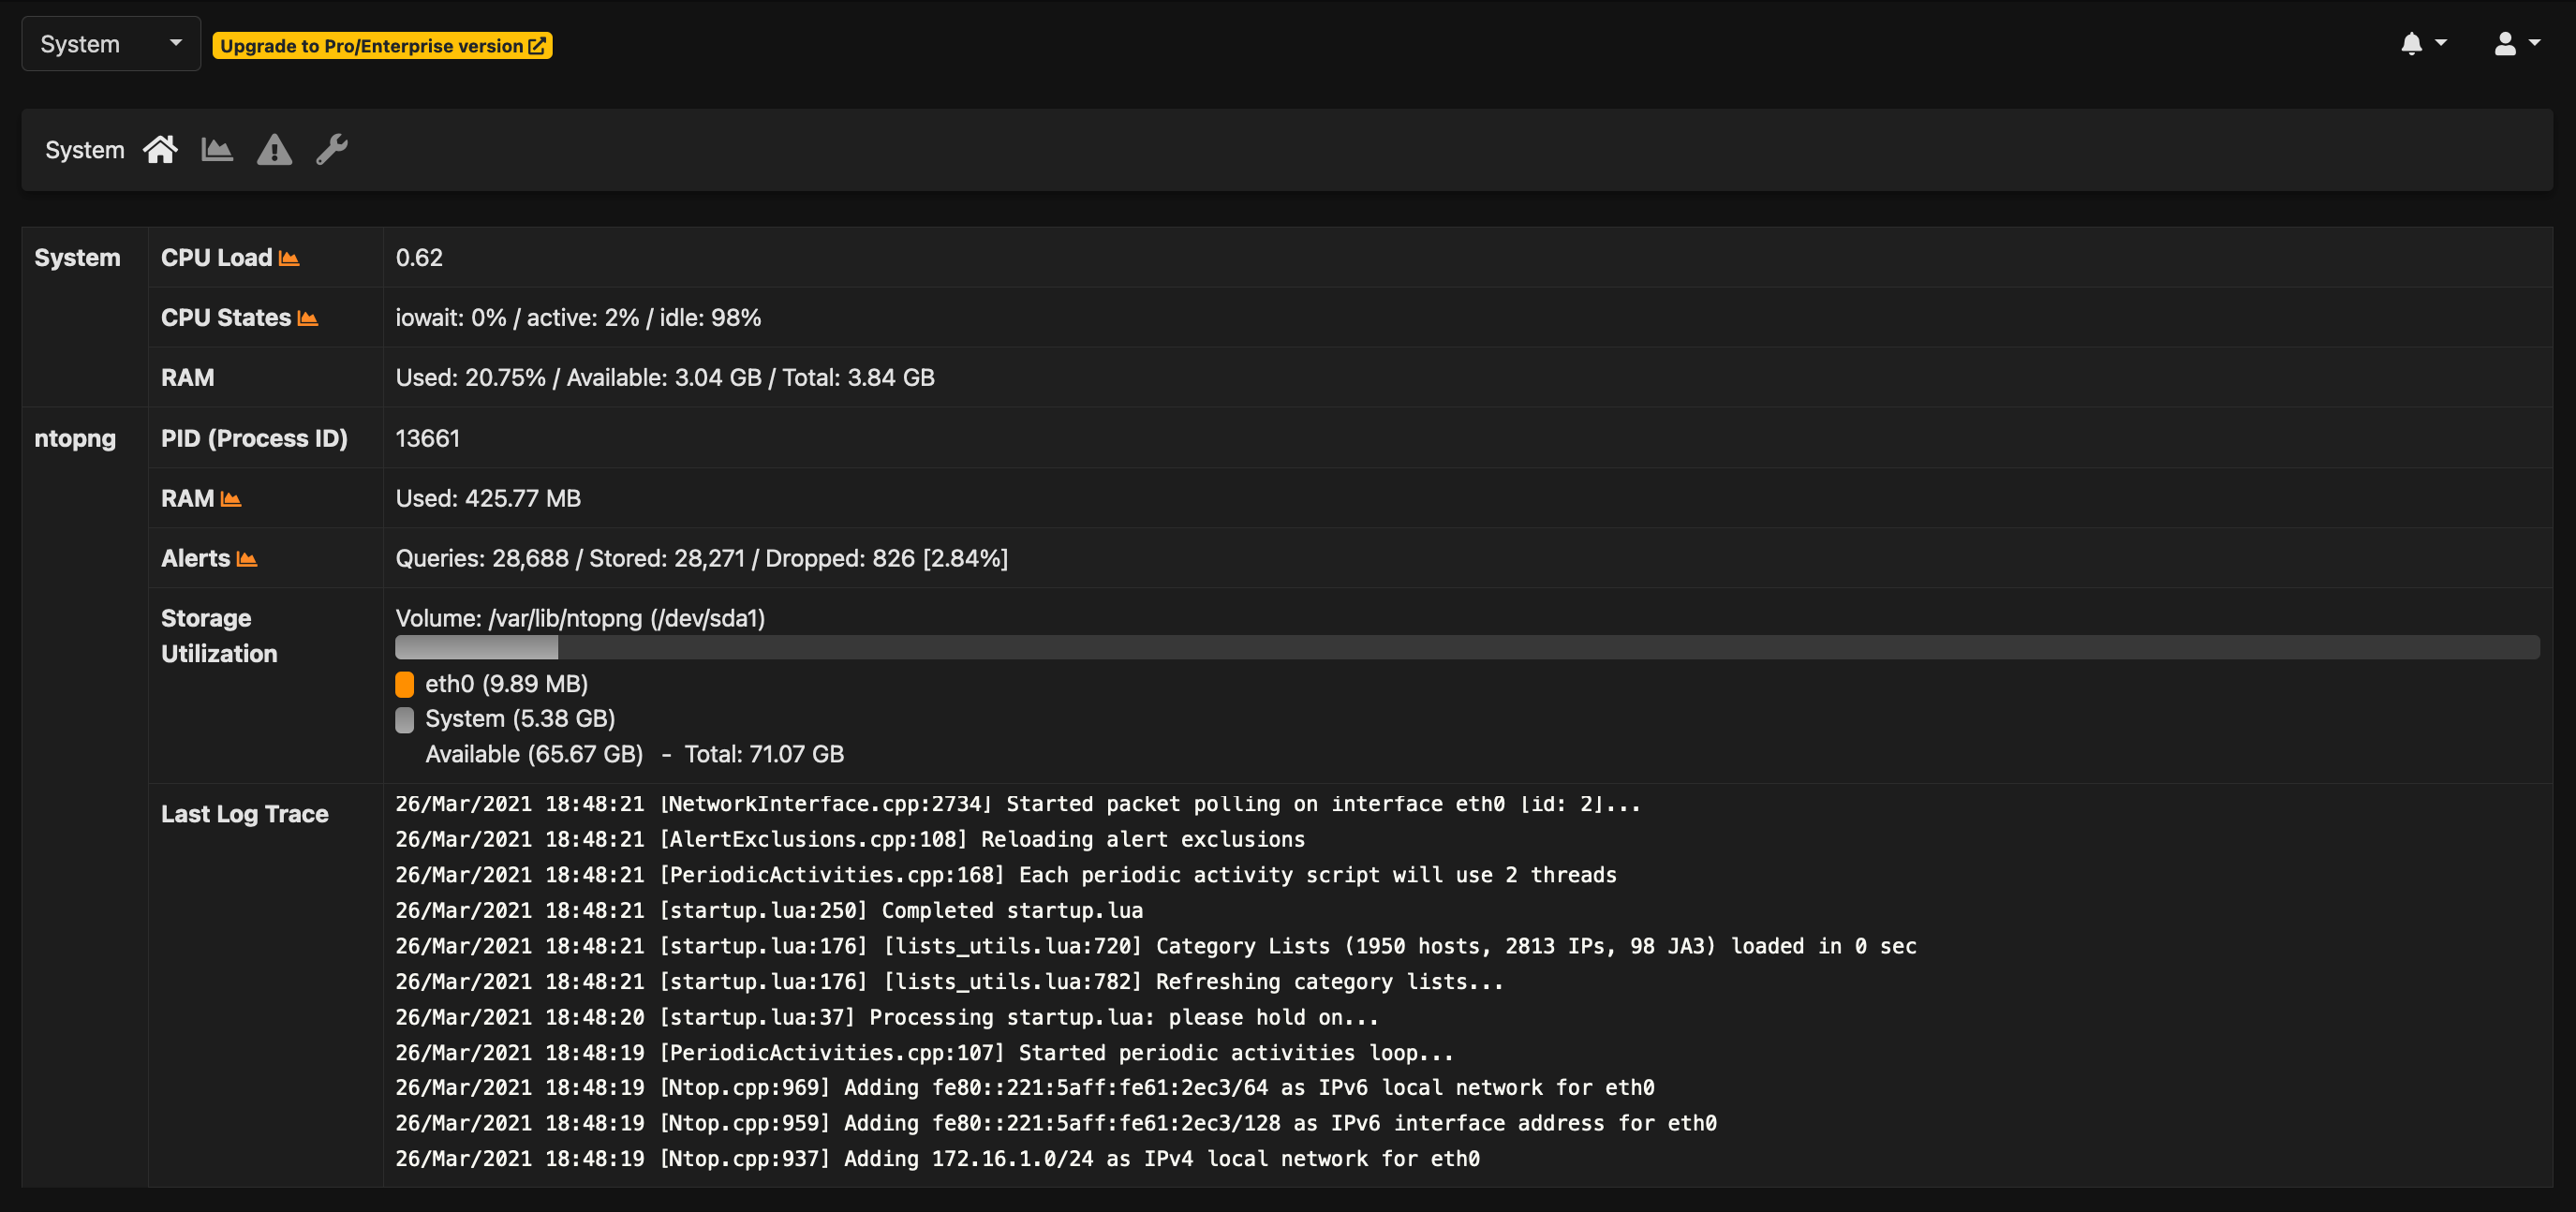
\includegraphics[width=.8\linewidth]{figs/setup/system.png}
    \caption{Utilização dos recursos do sistema}
    \label{fig:system}
\end{figure}

\section{Comparação}

Estas duas ferramentas e os resultados obtidos diferem em vários aspetos. Vamos analisar essas diferenças nesta secção.

\subsection{Monitorização de tráfego}

O NTOP, como mencionado anteriormente, regista todo o tráfego que usa a interface \textit{eth0}.
Esta interface é usada para praticamente todo tráfego, quer dentro da rede local quer externo.
Deste modo o NTOP é capaz de registar todo o tráfego dos serviços instalados no tux12.

O MRTG faz a monitorização do tráfego através do protocolo SNMP.
Ele foi configurado para monitorizar o router de bancada onde foi ativado o SNMP.
Pelas razões mencionadas na capítulo \ref{prop_rede}, o MRTG neste contexto não é capaz de ler todo o tráfego gerado pelos serviços, dado que nem todo o tráfego passa pelo router.
Desde modo, não é possível fazer uma análise total da utilização do nosso serviço com dois tipos de tráfego: \textit{Local->Local e Remote->Local}.

\subsection{User Interface}

O MRTG não faz distinção do tipo de tráfego.
De uma forma simples, apresenta gráficos com a evolução do tráfego total recebido e enviado ao longo do tempo.

O NTOP faz discriminação do tráfego, assim como da origem dele. Apresenta vários gráficos e tabelas onde podemos ver o tipo de tráfego, a sua origem, e a sua evolução ao longo do tempo.
Deste modo, podemos afirmar que o NTOP apresenta muita mais informação do que o MRTG.

Comparando os dois gráficos horários do NTOP (Fig \ref{fig:hourly}) e MRTG (Fig \ref{fig:mrtg_main}), pode-se observar que no MRTG não estão presentes os picos de tráfego em 100kB que vemos no NTOP.
Isto deve-se ao facto do tráfego FTP não estar a ser monitorizado. Estão a ser realizados acessos FTP do tipo \textit{Remote->Local}, um tipo de tráfego que não passa pelo router de bancada.
Para se poder observar tráfego FTP, seria necessário fazer ligações a servidores FTP da outra sala.
Isto não foi possível realizar em tempo útil, pois à data da recolha dos dados, não havia servidores FTP na outra sala disponíveis para este teste.

\subsection{Use Cases}
O NTOP provou ser a melhor ferramenta neste contexto. No entanto, não regista o tráfego utilizado por outras interfaces de outros \textit{tux}s.
Como na nossa configuração, todos os serviços estavam instados no \textit{tux12}, isto não foi um problema.

O MRTG é mais útil para monitorizar o tráfego de um servidor. Se estivéssemos a ler o switch, iríamos conseguir ver todo o tráfego \textit{Local->Local / Remote->Local / Local->Remote}.
Isto seria mais útil, sendo que estaríamos a ver todo o tráfego gerado por todos os hosts dentro da sala I321.

Ao ler router \textbf{firetux}, não íamos conseguir ver tráfego local.



\section{Conclusão}
\begin{frame}{Conclusão}{}
    \begin{itemize}
        \item Fundamentos teóricos da Tonalidade
        \item Algoritmos de deteção
        \begin{itemize}
            \item Krumhansl-Schmukler
        \end{itemize}
        \item Key Profiles
        \begin{itemize}
            \item Krumhansl
            \item Temperley
            \item etc.
        \end{itemize}
        \item Implementação em Python
        \begin{itemize}
            \item Music21
        \end{itemize}
        \item Análise de precisão
        \begin{itemize}
            \item Melhorias no algoritmo
        \end{itemize}
    \end{itemize}
\end{frame}

%%%%%%%%%%%%%%%%

%put in our emails..
{\aauwavesbg
\begin{frame}[plain,noframenumbering]
  \finalpage{
      {\Large Obrigado e esperamos que tenham gostado!}\\
      \vspace{5mm}
      Diogo Remião - \href{mailto:up201706373@edu.fe.up.pt}{{\tt up201706373@edu.fe.up.pt}}\\
      José Miguel Pinheiro - \href{mailto:up201706172@edu.fe.up.pt}{{\tt up201705172@edu.fe.up.pt}}\\
  }
\end{frame}}
%%%%%%%%%%%%%%%%

\end{document}
